\documentclass[times, utf8, zavrsni, numeric]{fer}
\usepackage{booktabs}
\usepackage{listings}
\usepackage{color}
\usepackage{url}
\usepackage{amsmath}

\definecolor{mygreen}{rgb}{0,0.6,0}
\definecolor{mygray}{rgb}{0.5,0.5,0.5}
\definecolor{mymauve}{rgb}{0.58,0,0.82}

\lstset{ %
  backgroundcolor=\color{white},   % choose the background color
  basicstyle=\footnotesize,        % size of fonts used for the code
  breaklines=true,                 % automatic line breaking only at whitespace
  captionpos=b,                    % sets the caption-position to bottom
  commentstyle=\color{mygreen},    % comment style
  escapeinside={\%*}{*)},          % if you want to add LaTeX within your code
  keywordstyle=\color{blue},       % keyword style
  stringstyle=\color{mymauve},     % string literal style
}

\begin{document}

\thesisnumber{4581}

\title{Očitavanje rukom pisanih slova}

\author{Filip Gulan}

\maketitle

% Ispis stranice s napomenom o umetanju izvornika rada. Uklonite naredbu \izvornik ako žlite izbaciti tu stranicu.
\izvornik

% Dodavanje zahvale ili prazne stranice. Ako ne želite dodati zahvalu, naredbu ostavite radi prazne stranice.
\zahvala{Zahvaljujem se mentoru doc.\ dr.\ sc.\ Marku Čupiću na velikoj pomoći i strpljenju prilikom izrade završnog rada te svim prijateljima i kolegama koji su sudjelovali u izradi skupa podataka rukom pisanih znakova.}

\tableofcontents

\chapter{Uvod}
Zahtjev za svakodnevnom obradom sve veće količine podataka polako, ali sigurno, stvara velik problem čovjeku. Svaki dan zahtjeva se obrada ogromne količine papirnatih dokumenata koje je uglavnom potrebno obraditi i unijeti na računalo. Kako bi se izbjeglo ručno prepisivanje projektiraju se raznorazni sustavi koji će taj posao automatizirati.

Primjer jednog takvog posla je i ispravljanje provjera znanja s abc-pitalicama. Ispitanik svoj odgovor unosi zacrnjivanjem u matrici za unos odgovora. No u slučaju pogreške, ispitanik može promijeniti odgovor tako da izravno upiše novi odgovor na za to odgovarajuće mjesto. Ukoliko bi jedan ispravljač ručno provjeravao svaki obrazac i unosio u sustav, taj bi posao na kolegijima od 600 i više studenata trajao i po nekoliko dana.

Kroz ovaj rad pokazat će se implementacija sustava za prepoznavanje rukom pisanih slova koji će na svoj ulaz primiti izdvojenu sliku slova te kao rezultat vratiti prepoznato slovo. Prvi korak će biti prikupljanje skupa podataka rukom pisanih slova, zatim obrada istih. Nakon toga slijedi izgradnja sustava za klasifikaciju pojedinog slova te njegovo iskorištavanje u stvarnim uvjetima rada.

Kao sustav za klasifikaciju bit će korištena umjetna neuronska mreža učena algoritmom propagacije pogreške unatrag. Razlog tomu je jednostavna implementacija takvog sustava te velika sposobnost generalizacije koje nudi neuronska mreža. Kako dobivena slika slova može biti velika i neobrađena, prije prikazivanja podataka neuronskoj mreži, sliku je potrebno obraditi te izvući vektor značajki. Prilikom izlučivanja vektora značajki koristiti će se dijagonalna projekcija, koja je relativno nov pojam predstavljen u radu \citep{diagonal2011}. 

Ostatak rada organiziran je kako slijedi. U drugom poglavlju opisan je postupak prikupljanja i obrade skupa podataka. U trećem poglavlju opisan je postupak klasifikacije korištenjem neuronske mreže koja je učena algoritmom propagacije pogreške unatrag uz dodatak momenta inercije. U četvrtom poglavlju su predstavljene metode izlučivanja značajki iz pojedinog slova dok su u petom poglavlju predstavljeni usporedni rezultati učenja neuronske mreže korištenjem različitih metoda izlučivanja značajki.

\chapter{Obrada slike}
Prvi korak pri prepoznavanju rukom pisanih slova sastoji se od prikupljanja skupa podataka te obrade istoga. Obrada se sastoji od niza provedenih transformacija i filtra nad danim dokumentom, poput izdvajanja pojedinog slova, pretvaranja slike u sive nijanse, binarizacije, dilatacije, rezanja, skaliranja te stanjivanja \engl{thinning}. Cijeli postupak je prikazan na slici \ref{fig:image_process_flow}.
\begin{figure}[htb]
\centering
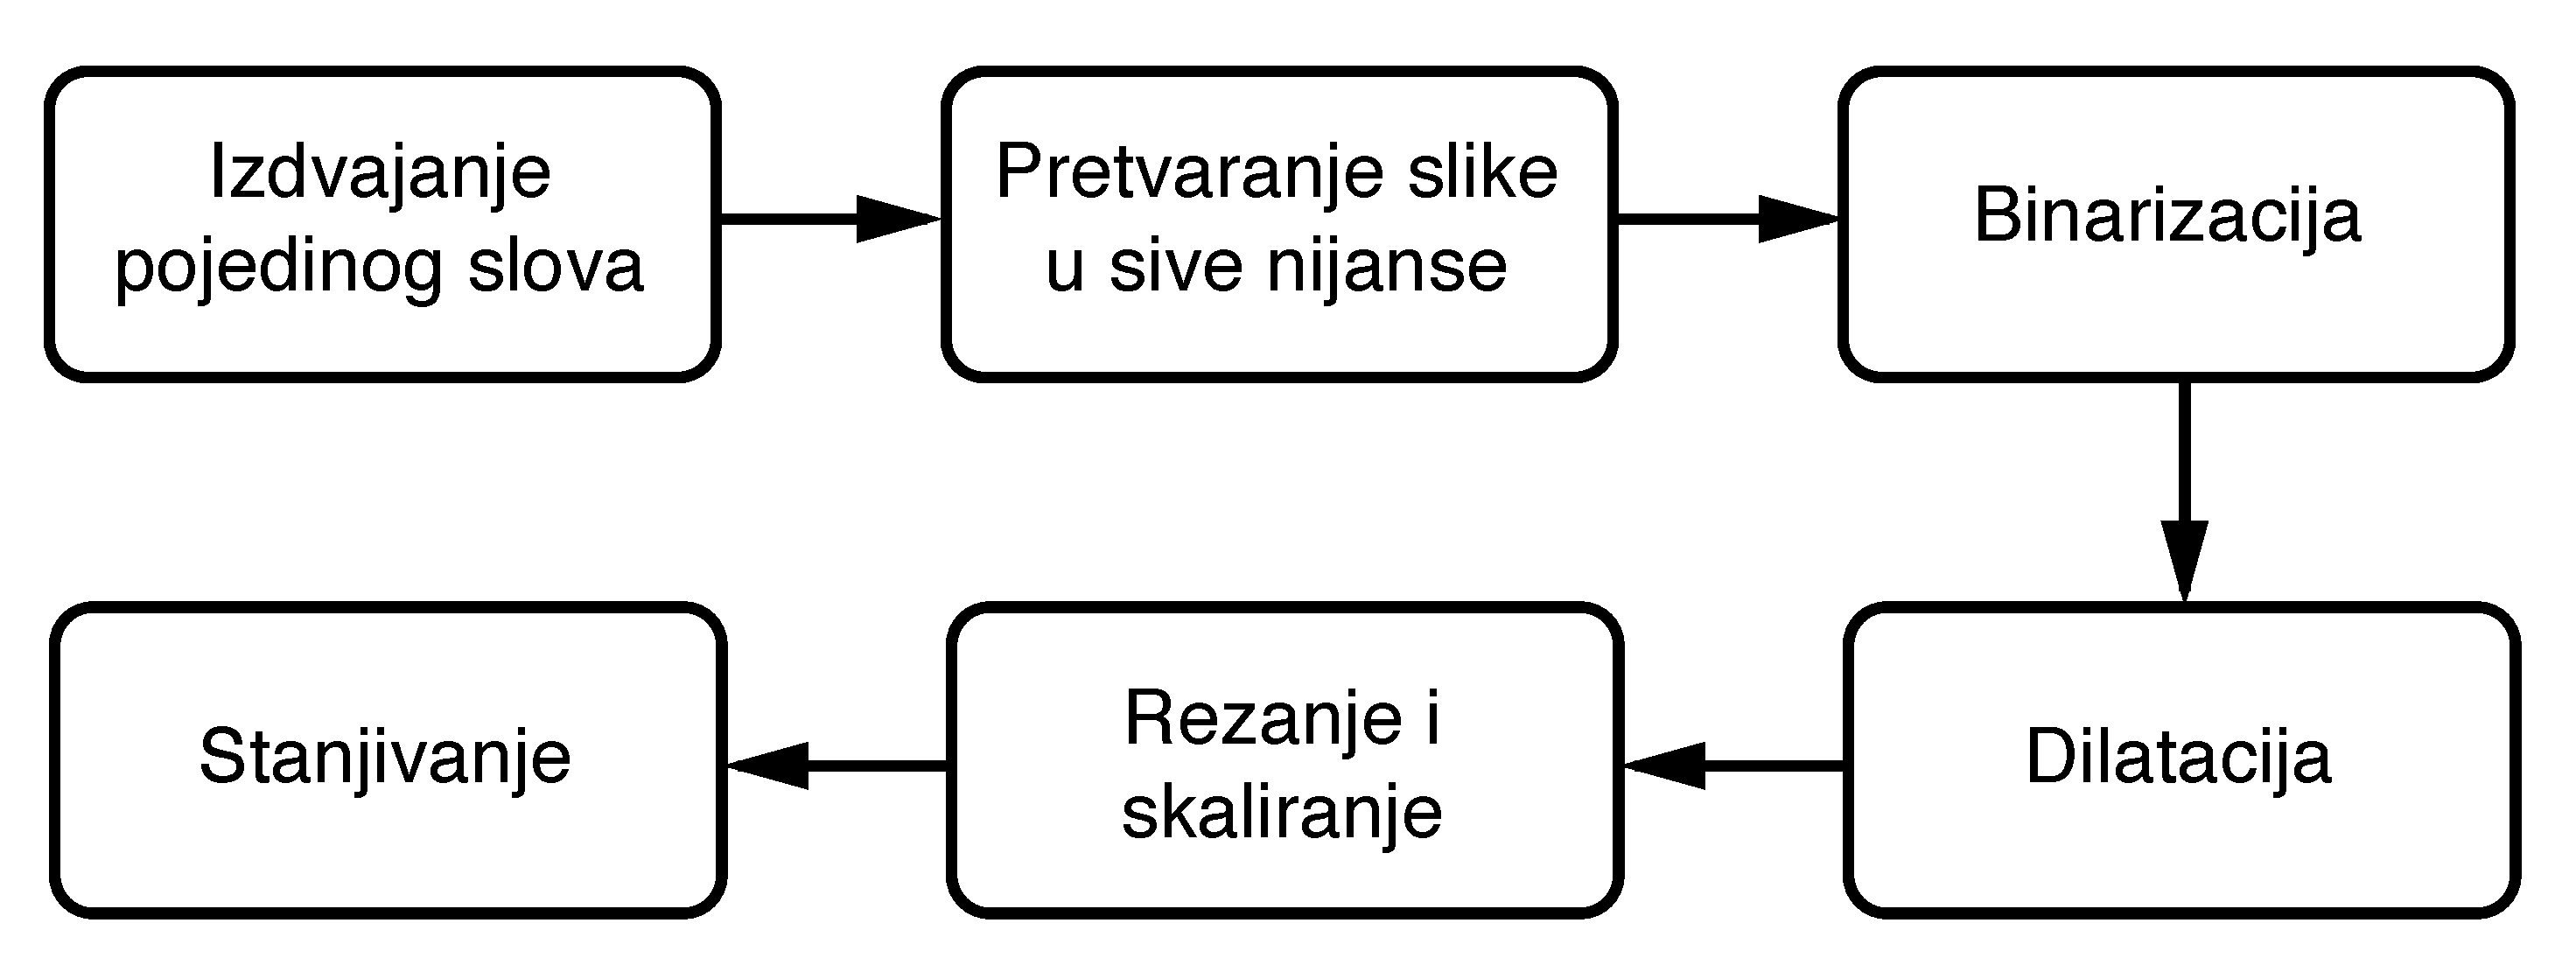
\includegraphics[width=12cm]{images/image_process_flow.pdf}
\caption{Postupak obrade slike}
\label{fig:image_process_flow}
\end{figure}

\section{Prikupljanje skupa podataka}
Prikupljanje rukom pisanih slova se obavljalo pomoću obrasca, prikazanog na slici \ref{fig:obrazac}, na kojem je trebalo ispisati po pet varijanti velikog i malog tiskanoga slova hrvatske i engleske abecede te dodatnog znaka '-' koji bi u sustavima za automatsko ocjenjivanje odgovora služio kao znak za poništavanje danog odgovora. Prostor za unos pojedinog slova je kvadratnih dimenzija kako bi se kasnije olakšalo izdvajanje pojedinog slova 
Za daljnje izdvajanje pojedinog slova iz obrasca koristio se alat \emph{Sketch}, dostupan samo za \emph{OS X} operacijski sustav. \emph{Sketch} se uglavnom koristi za razvoj dizajna za mobilne aplikacije (\emph{iOS, Android}), no za potrebe ovog rada se pokazao vrlo praktičnim jer nudi definiranje regija na slici koje je moguće sve skupa odjednom izrezati, te svaku regiju spremiti u zasebnu datoteku. Pri obradi svakog novog obrasca trebalo je samo mijenjati pozadinu, to jest obrazac, dok bi regije zadržale svoj položaj.

Za potrebe pisanja ovog rada prikupljeno je sedamnaest obrazaca, od kojih su dvoje ispisani grafitnom olovkom pa je skenirani oblik bio vrlo loše kvalitete, i jedan na ćirilici. Obrasci su skenirani u boji te su na računalu prebačeni u nijanse sive boje. Razlog tomu je loša implementacija filtra sivih tonova na skenerima, što će biti objašnjeno u sljedećem potpoglavlju.
\begin{figure}[htb]
\centering
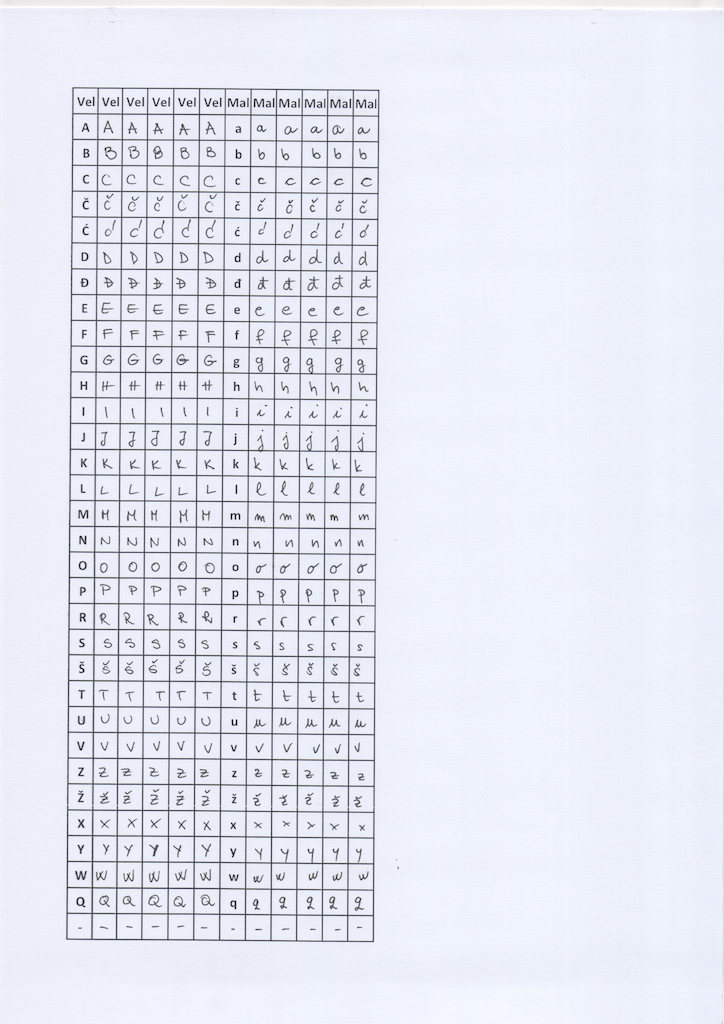
\includegraphics[width=8cm]{images/obrazac.png}
\caption{Obrazac za prikupljanje rukom pisanih slova}
\label{fig:obrazac}
\end{figure}

\section{Pretvaranje boje u nijanse sive}
Prvi korak nakon izdvajanja pojedinog slova je pretvaranje boje u nijanse sive. U svakodnevnoj uporabi se nalazi nekoliko algoritama \citep{grayscaleAlg} i većinom su vrlo jednostavni za implementirati.

Za početak nužno je shvatiti kako računalo koristi i prikazuje boje. Za prikaz boja koristi se aditivni model RGB \engl{Red Green Blue}, koji stapanjem u određenim omjerima, crvene, zelene i plave boje daje ostale boje vidljivog spektra. Tako izostanak sve tri boje, to jest prisutnost u omjeru $0:0:0$, daje crnu boju dok prisutnost svih boja u omjeru $1:1:1$ daje bijelu boju. 

Može se uočiti, ukoliko su sve tri komponente u podjednakim omjerima dobiva se boja koja se nalazi u spektru između crne i bijele boje, što je zapravo spektar sivih nijansi. Stoga se svi algoritmi za pretvorbu boja u nijanse sive temelje na pristupu gdje su sve tri komponente podjednako raspoređene.

Prvi algoritam je vrlo jednostavan i intuitivan. Siva nijansa pojedinog slikovnog elementa se dobiva tako da se boja slikovnog elementa rastavi na tri navedene komponente. Omjer pojedinih komponenti se zbraja te se uzima srednja vrijednost, kako je prikazano izrazom \eqref{eq:uniform_grayscale}.
\begin{equation} \label{eq:uniform_grayscale}
E_y = \frac{E_R + E_G + E_B}{3}
\end{equation}

Prikaz rada algoritma je vidljiv na slici \ref{fig:grayscale_uniform_example}. Algoritam je intuitivan i vrlo jednostavan, no u praksi ne daje najbolje rezultate. Problem leži u ljudskom oku i načinu na koji opaža boje. Ljudsko oko zelenu boju opaža puno jače nego crvenu, te crvenu opaža jače nego plavu.

\begin{figure}[htb]
    \centering
    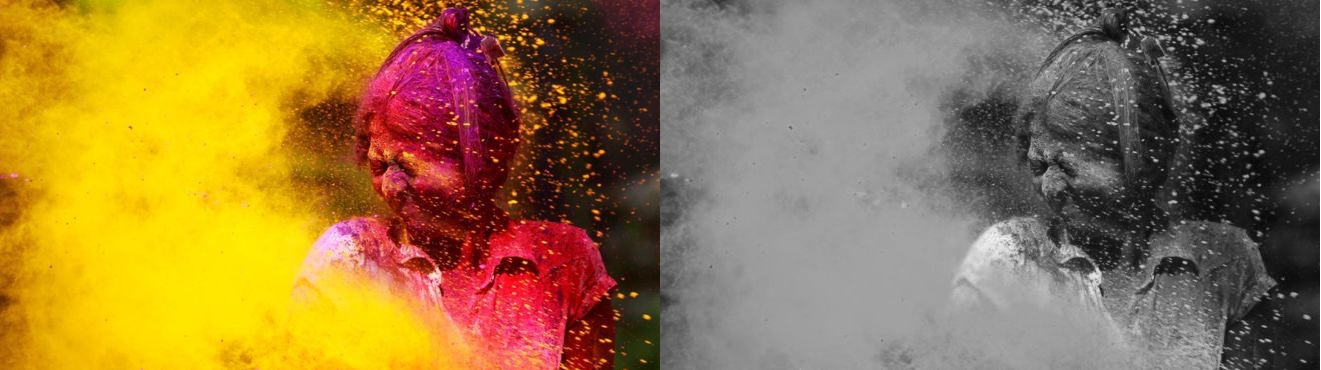
\includegraphics[width=14.5cm]{images/grayscale_uniform_example_h.jpg}
    \caption{Prikaz rada prvog algoritma pretvorbe boja u nijanse sive, preuzeto iz \citep{grayscaleImg}}
    \label{fig:grayscale_uniform_example}
\end{figure}

Na slici \ref{fig:grayscale_uniform_example}, na dijelu koji je u boji, vrlo jasno se opaža žuta boja, no pretvorbom slike u sive tonove uporabom prvog algoritma dobiva se dojam kao da se žuta boja stopila s pozadinom. Žuta boja je sastavljena od tri navedene komponente u omjeru $1:1:0$, te je predloženi algoritam zapravo u jednakom omjeru "pomiješao" zelenu i crvenu komponentu što se kosi sa načinom na koji ljudsko oko opaža boje.

Stoga intuitivno slijedi da bi zelena trebala biti najzastupljenija, zatim crvena i plava. Organizacija ITU \engl{International Telecommunication Union} u svojoj normi ITU-R BT.709-6 \citep{ITUgrayscale} predlaže drugi algoritam u kojem bi crvena komponenta imala udio s 22.16\%, zelena s 71.56\% te plava s 7.22\%, što je prikazano izrazom \eqref{eq:itu_grayscale}.
\begin{equation} \label{eq:itu_grayscale}
E_y = 0.2126E_R + 0.7152E_G + 0.0722E_B
\end{equation}

Izraz \eqref{eq:itu_grayscale} se često može naći u literaturi pod imenom \emph{Luma} te daje mnogo bolje rezultate nego izraz \eqref{eq:uniform_grayscale}. Na slici \ref{fig:grayscale_example_all} mogu se usporediti rezultati obadva izraza, gdje je jasno vidljiva prednost korištenja izraza \eqref{eq:itu_grayscale}.

\begin{figure}[htb]
    \centering
    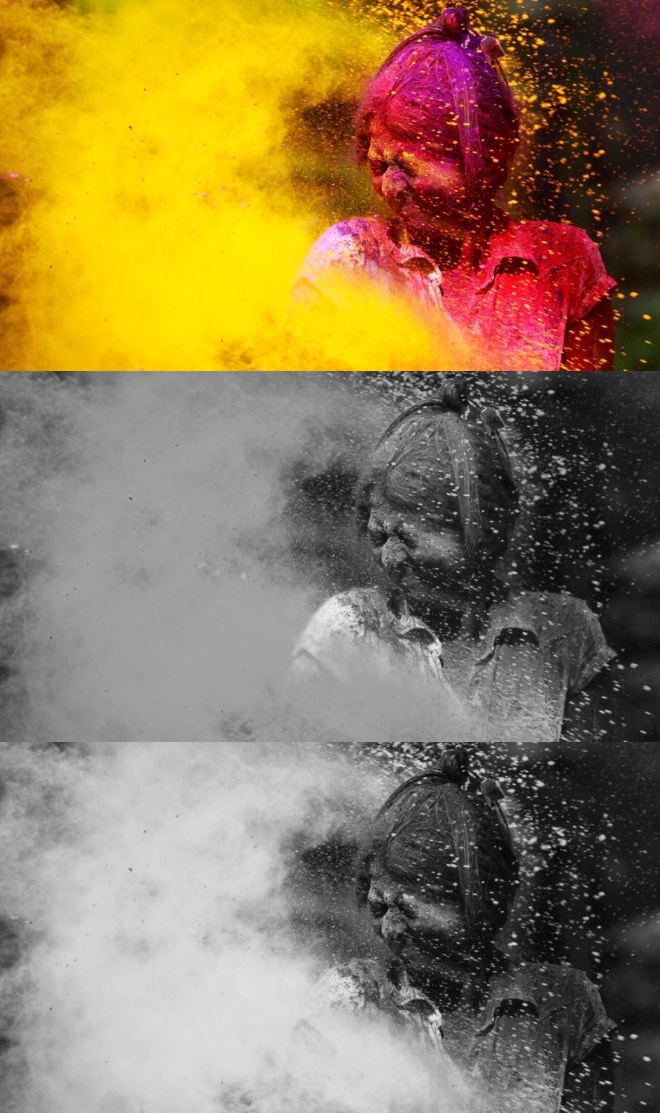
\includegraphics[width=9cm]{images/grayscale_example_all.jpg}
    \caption{Usporedba prvog i drugog algoritma pretvorbe boja u nijanse sive}
    \label{fig:grayscale_example_all}
\end{figure}

Za potrebe ovog rada korišten je izraz \eqref{eq:itu_grayscale}. Sama obrada obrasca i pretvorba u nijanse sive mogla se napravit prilikom skeniranja, no nije iz razloga što većina današnjih skenera i digitalnih kamera koristi treći algoritam koji je zapravo najjednostavnijih od svih i daje najlošije rezultate. Skener ili digitalna kamera se sastoji od senzora za pojedinu komponentu, to jest crvenu, zelenu i plavu. Pri pretvorbi boje u nijanse sive, skener ili kamera, kako ne bi trebao vršiti bilo kakvo računanje, odabire jednu komponentu i proglašava trenutnu vrijednost te komponente kao nijansu sive. U većini slučajeva je to zelena komponenta, zbog već spomenutog načina na koji ljudsko oko opaža boje.

Prikaz rada algoritma uporabom izraza \eqref{eq:itu_grayscale} nad skeniranim slovom vidljiv je na slici \ref{fig:grayscale_char_example}.

\begin{figure}[htb]
    \centering
    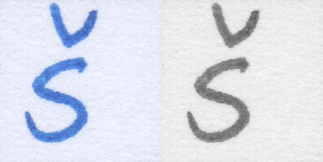
\includegraphics[width=8cm]{images/char_grayscale_example.png}
    \caption{Prikaz rada drugog algoritma nad skeniranim slovom}
    \label{fig:grayscale_char_example}
\end{figure}

Implementacija kompletnog rješenja pretvorbe slike u nijanse sive uporabom izraza \eqref{eq:itu_grayscale} u programskom jeziku \emph{Java} dana je sljedećim izvornim kodom.
\lstset{language=Java, tabsize=2}
\begin{lstlisting}
public BufferedImage applyFilter(BufferedImage sourceImage) {
        int width = sourceImage.getWidth();
        int height = sourceImage.getHeight();
        BufferedImage filteredImage = new BufferedImage(width, height, sourceImage.getType());

        int gray, rgb;
        for (int i = 0; i < width; i++) {
            for (int j = 0; j < height; j++) {
                rgb = sourceImage.getRGB(i, j);
                gray = getGray(ImageUtilities.getRed(rgb),
                        ImageUtilities.getGreen(rgb),
                        ImageUtilities.getBlue(rgb));

                gray = ImageUtilities.
                        colorToRGB(255, gray, gray, gray);
                filteredImage.setRGB(i, j, gray);
            }
        }
        return filteredImage;
    }
    
    private int getGray(int red, int green, int blue) {
        return Math.round(0.2126f * red +
                0.7152f * green +
                0.0722f * blue);
    }
\end{lstlisting}

Nakon pretvaranja boja u nijanse sive slijedi binarizacija dobivene slike slova.

\section{Binarizacija}
Binarizacija je postupak kojim se slika sivih nijansi pretvara u crno-bijelu sliku. Sam postupak binarizacije je vrlo jednostavan. Odabere se prag binarizacije, to jest vrijednost sive nijanse iznad koje će se slikovni element smatrati bijelim, a ispod te vrijednosti crnim. 

Kako bi se izbjegla ovisnost o pragu binarizacije, koristi se \emph{Otsu-ova} metoda binarizacije \citep{1979:ots}, koja prag određuje dinamički. Osnova na kojoj se temelji navedena metoda je korištenje histograma slike uz pretpostavku da slika sadrži dvije klase slikovnih elemenata, pozadinu i prednji plan, to jest u slučaju ovog rada slovo i pozadinu, kako je i prikazano na slici \ref{fig:histogram}.
\begin{figure}[htb]
    \centering
    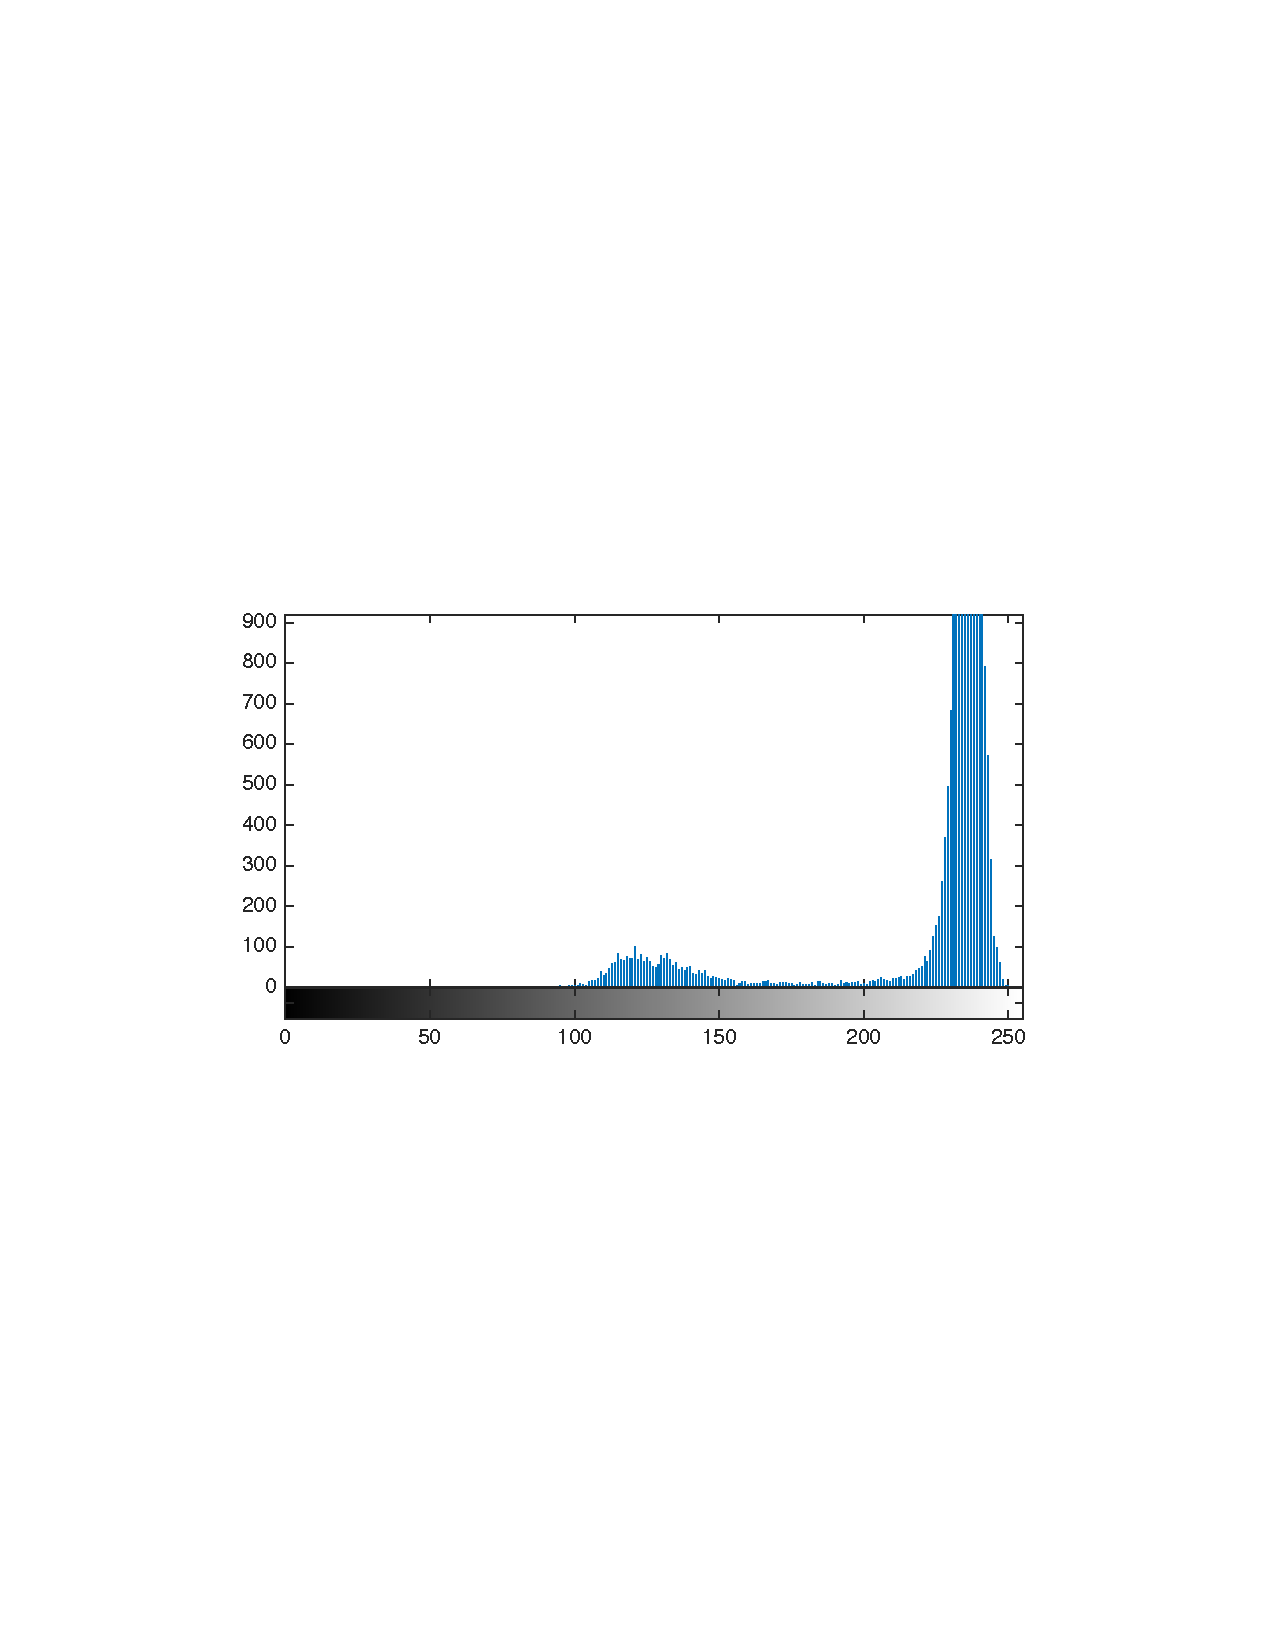
\includegraphics[width=12cm]{images/histogram.pdf}
    \caption{Histogram sive slike}
    \label{fig:histogram}
\end{figure}

Prvi korak je izračun histograma slike koji će se koristiti u daljnjim koracima. Otsu je u svojoj metodi pokazao da je klase moguće odijeliti korištenjem histograma slike i disperzije unutar i između razreda. Za svaki prag $t$ računa se disperzija unutar razreda i vrijednost pri kojoj je minimalna odabire se za prag binarizacije:
\begin{equation} \label{eq:within_class}
    \sigma_w^2(t) = \omega_0(t)\sigma_0^2(t) + \omega_1(t)\sigma_1^2(t),
\end{equation}
gdje su $\omega_0(t)$ i $\omega_1(t)$ definirane kao vjerojatnosti pojave, to jest udio prednjeg plana i pozadine:
\begin{align}
    \omega_0(t)&=\sum_{i=0}^{t-1}p(i), \label{eq:background} \\
    \omega_1(t)&=\sum_{i=t}^{L-1}p(i)=1-\omega_0(t), \label{eq:foreground}
\end{align}
ukoliko se intezitet nijansi sive boje kreće u rasponu $[0, L-1]$, a $p(i)$ predstavlja vjerojatnost pojave određene komponente $i$ u histogramu sive slike, gdje je $i \in [0, 255]$. $p(i)$ je definiran izrazom \eqref{eq:histogram_p_i}.
\begin{equation} \label{eq:histogram_p_i}
    p(i) = \dfrac{histogram(i)}{\sum_{j=0}^{L-1}histogram(j)}
\end{equation}

Računanje disperzije unutar razreda je složeno i zahtjeva mnogo računskih operacija. No maksimizacija disperzije između razreda ekvivalentna je minimizaciji disperzije unutar razreda stoga je izračun disperzije između razreda češće korišten oblik, pogotovo pri implementaciji na računalu. Matematički opisano to izgleda ovako \citep{1979:ots}:
\begin{equation} \label{eq:between_class}
    \sigma_b^2(t) = \sigma^2 - \sigma_w^2(t) = \omega_0(t)\omega_1(t)(\mu_1(t) - \mu_0(t))^2,
\end{equation}
gdje su $\mu_0(t)$ i $\mu_1(t)$ očekivanja pojedinog razreda definirana kao:
\begin{align}
    \mu_0(t)&=\sum_{i=0}^{t-1}\frac{i\cdot p(i)}{\omega_0(t)}, \label{eq:mean_bg} \\
    \mu_1(t)&=\sum_{i=t}^{L-1}\frac{i\cdot p(i)}{\omega_1(t)}, \label{eq:mean_fg}
\end{align}

Implementacija izračuna \emph{Otsu-ovog} praga u programskom jeziku \emph{Java} prikazana je sljedećim izvornim kodom.
\lstset{language=Java, tabsize=2}
\begin{lstlisting}
    private int threshold(int[] histogram, int size) {
        float sum = 0, varMax = 0, sumB = 0;
        for (int i = 0; i < 256; i++) {
            sum += i * histogram[i];
        }
        int wB = 0, wF = 0, threshold = 0;;

        for (int i = 0; i < 256; i++) {
            wB += histogram[i];
            if (wB == 0) continue;
            wF = size - wB;
            if (wF == 0) break;

            sumB += (float) (i * histogram[i]);
            float mB = sumB / wB;
            float mF = (sum - sumB) / wF;

            float varBetween = (float) wB * (float) wF * (mB - mF) * (mB - mF);
            if (varBetween > varMax) {
                varMax = varBetween;
                threshold = i;
            }
        }
        return threshold;
    }
\end{lstlisting}

Prikaz rada algoritma binarizacije uporabom Otsuove metodom otkrivanja praga prikazan je na slici \ref{fig:binarization_example}.

\begin{figure}[htb]
    \centering
    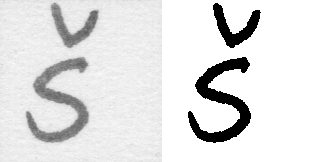
\includegraphics[width=8cm]{images/binarization_example.png}
    \caption{Prikaz rada algoritma binarizacije nad sivom slikom}
    \label{fig:binarization_example}
\end{figure}

Sljedeći korak je dilatacija binarne slike, kojeg nije nužno uvijek provesti, već ovisi o samoj kvaliteti dostupnog skupa podataka.

\section{Dilatacija}
Dilatacija je jedan od osnovnih operatora u području matematičke morfologije. Obično se primjenjuje na binarnim (crno-bijelim) slikama, no postoje i verzije algoritma koje rade i za slike sivih nijansi. Laički rečeno, dilatacija služi za podebljavanje te popunjavanje sitnih nepravilnosti i praznina unutar prednjeg plana, što može bitno utjecati na daljnju obradu slike. Matematički, dilatacija je definirana kao
\begin{equation} \label{eq:dilation}
    D(\textbf{A, B}) = \textbf{A} \oplus \textbf{B} = \bigcup_{b \in \textbf{B}} \textbf{A}_b.
\end{equation}
Skup \textbf{A} predstavlja sliku, to jest skup točaka koje pripadaju slici, nad kojom se vrši dilatacija, dok je skup \textbf{B} operator koji se naziva strukturni element, odnosno skup točaka strukturnog elementa, u literaturi često naveden pod imenom jezgra \engl{kernel}, i on je jezgra algoritma dilatacije. Strukturni element može biti raznih oblika, od kruga do kvadrata, te on određuje vrstu i svojstva dilatacije.

Za potrebe ovog rada korišten je kvadratni strukturni element dimenzija $3 \times 3$ prikazan na slici \ref{fig:kernel}. Na slici \ref{fig:kernel} oznaka '1' označava crni slikovni element. Element označen crvenom bojom predstavlja centralni element kojim se vrši usporedba s izvornom slikom.
\begin{figure}[htb]
    \centering
    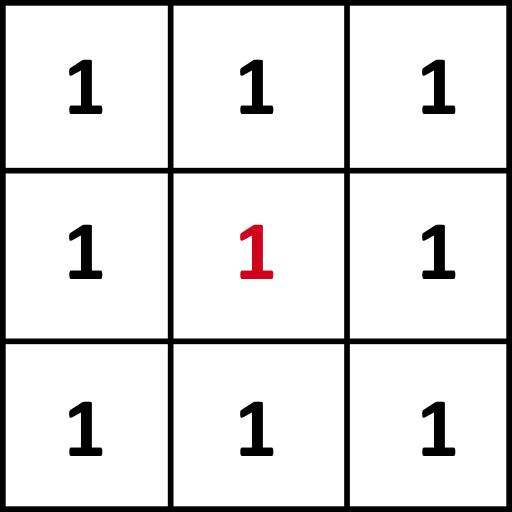
\includegraphics[width=4cm]{images/3x3kernel.jpg}
    \caption{Strukturni element dimenzija 3x3}
    \label{fig:kernel}
\end{figure}

Sam algoritam dilatacije je vrlo intuitivan i jednostavan za implementaciju. Iznad originalne slike postavi dani strukturni element, prikazan na slici \ref{fig:kernel}, te se iterira po pojedinom slikovnom elementu. Zatim, ukoliko se centralni element nađe iznad crnog slikovnog elementa originalne slike, na novoj slici se oboja u crno slikovni element koji se nalazi na koordinati na kojoj se nalazi centralni element te svih ostalih osam susjednih elemenata. Implementacija danog algoritma u programskom jeziku \emph{Java} prikazano je sljedećim izvornim kodom \citep{Gonzalez}.
\lstset{language=Java, tabsize=2}
\begin{lstlisting}
public BufferedImage applyFilter(BufferedImage sourceImage) {
    width = sourceImage.getWidth();
    height = sourceImage.getHeight();
    
    BufferedImage filteredImage = clone(sourceImage);
    for (int i = 0; i < width; i++) {
        for (int j = 0; j < height; j++) {
            int color = ImageUtilities.
                    getRed(sourceImage.getRGB(i, j));
            if (color == BLACK) {
                convolve(i, j, sourceImage);
            }
        }
    }
    return filteredImage;
}
// Konvoluiraj sliku strukturnim elementom
private void convolve(int i, int j, BufferedImage sourceImage, BufferedImage filteredImage) {
    for (int x = i - 1; x <= i + 1; x++) {
        for (int y = j - 1; y <= j + 1; y++) {
            if (x >= 0 && y >= 0 && x < width && y < height) {
                int rgb = ImageUtilities.
                        colorToRGB(255, 0, 0, 0);
                filteredImage.setRGB(x, y, rgb);
            }
        }
    }
}
\end{lstlisting}

Prikaz rada algoritma dilatacije vidljiv je na slici \ref{fig:dilation_good_example}. Bitno je primijetiti kako dano slovo ima sitnu nepravilnost u prednjem planu te bi ta nepravilnost dovela do velikih pogrešaka kod algoritma izvlačenja kostura slova, no dilatacija to uspješno rješava.
\begin{figure}[htb]
    \centering
    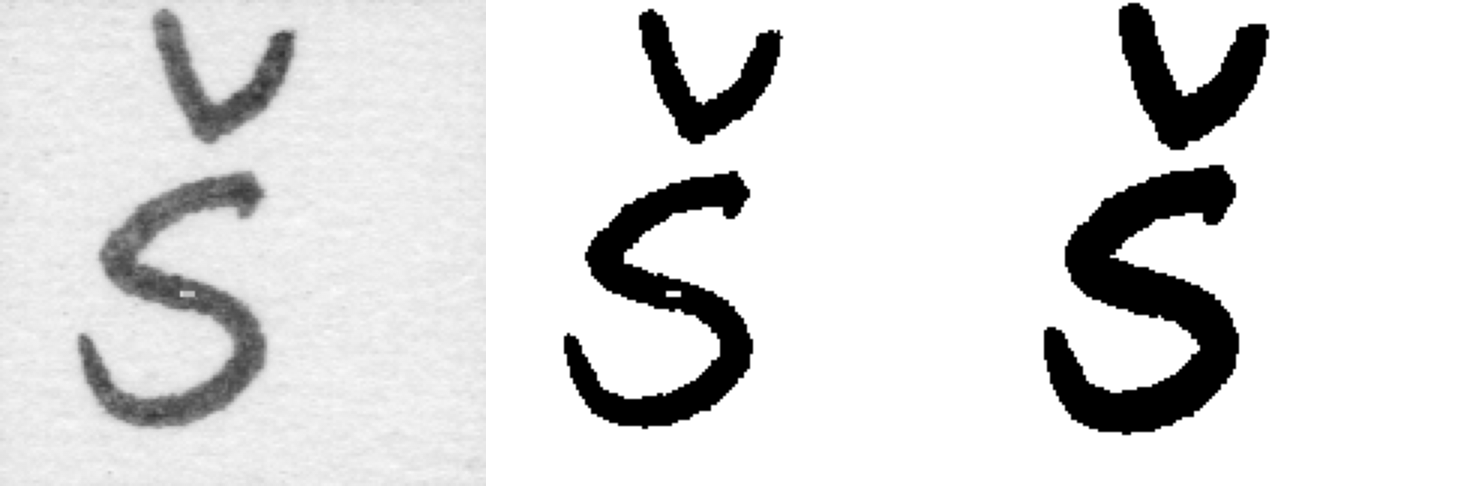
\includegraphics[width=10cm]{images/dilation_example.png}
    \caption{Prikaz rada algoritma binarizacije i dilatacije}
    \label{fig:dilation_good_example}
\end{figure}

Ukoliko dilatacija ne daje dobre rezultate u prvom prolazu, to jest još uvijek ostanu sitne praznine ili nepovezani dijelovi, može se ponoviti više prolaza. No time se gubi velika količina informacija o rukom pisanom slovu, što nikako nije poželjno.
\begin{figure}[htb]
    \centering
    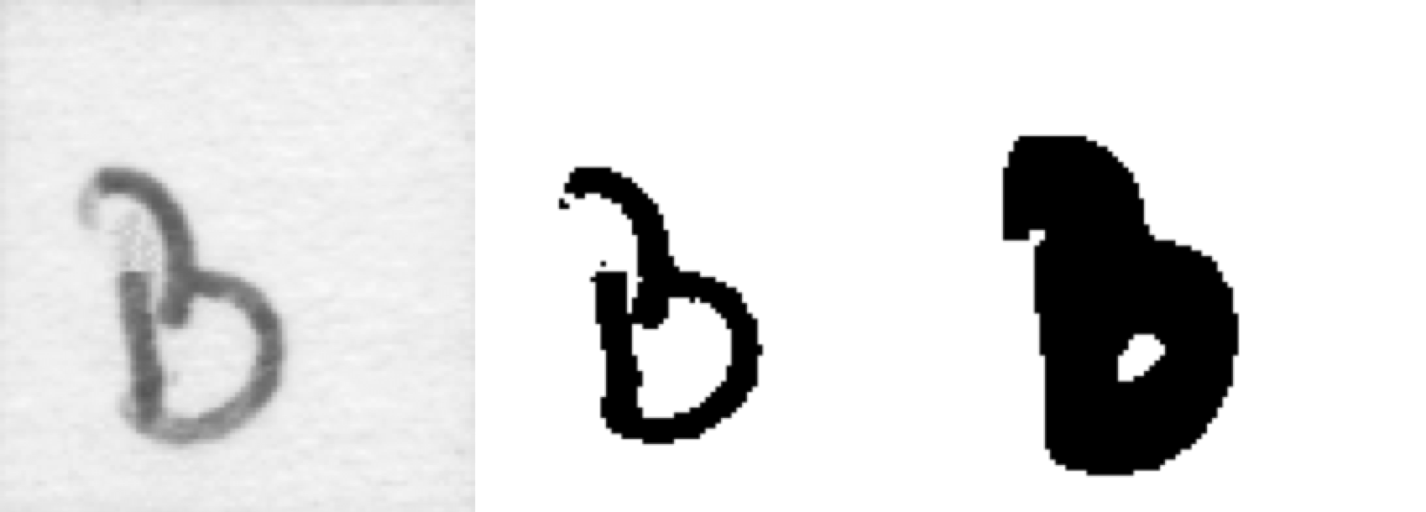
\includegraphics[width=10cm]{images/dilation_bad_example.png}
    \caption{Prikaz više prolaza algoritma dilatacije}
    \label{fig:dilation_bad_example}
\end{figure}
Dani problem se vidi na slici \ref{fig:dilation_bad_example} gdje je nakon tri prolaza algoritma dilatacije slovo 'B' neprepoznatljivo.

Sljedeći postupak je izvlačenje kostura slova, to jest stanjivanje \engl{thinning}.

\section{Stanjivanje}

Stanjivanje \engl{thinning} je jedna od osnovnih operacija u području matematičke morfologije. Poput dilatacije, obično se primjenjuje na binarnim (crno-bijelim) slikama, no postoje i verzije algoritma koje rade i za slike sivih nijansi. Operacija stanjivanja ima višestruku primjenu, no najčešće se koristi za izlučivanje kostura objekta, debljine jednog slikovnog elementa. U literaturi i na Internetu se stanjivanje i izlučivanje kostura vrlo često koriste kao sinonimi. Rezultat provedbe stanjivanja nad binarnom slikom je binarna slika.

U matematičko smislu, kao i kod dilatacije, stanjivanje je operacija nad skupom točaka koji pripadaju slici te skupom točaka koji provodi stanjivanje, to jest već prije spomenuti strukturni element. Jednostavan algoritam bi bio sljedeći: potrebno je uzeti u obzir sve slikovne elemente objekta, odnosno prednjeg plana, koji za susjeda imaju više od jednog slikovnog elementa koji pripada pozadini, zatim obrisati sve te elemente, ali samo u slučaju ukoliko neće doći do lokalnog razdvajanja objekta u dva dijela. Navedeni postupak ponavljati sve dok rezultat ne konvergira, to jest više se ne obriše niti jedan slikovni element u pojedinoj iteraciji algoritma. Ovaj postupak briše vanjske granice objekta, ali ne utječe na slikovne elemente na samim krajevima linija.

Navedeni algoritam se u morfologiji obavlja pomoću dva kvadratna strukturna elementa dimenzija $3 \times 3$, prikazanih na slici \ref{fig:thinning_el}, te svim njihovim rotacijama za 90 stupnjeva, što zapravo daje osam strukturnih elemenata. Element označen crvenom bojom predstavlja centralni element, to jest element kojim se vrši usporedba s originalnom slikom.
\begin{figure}[htb]
    \centering
    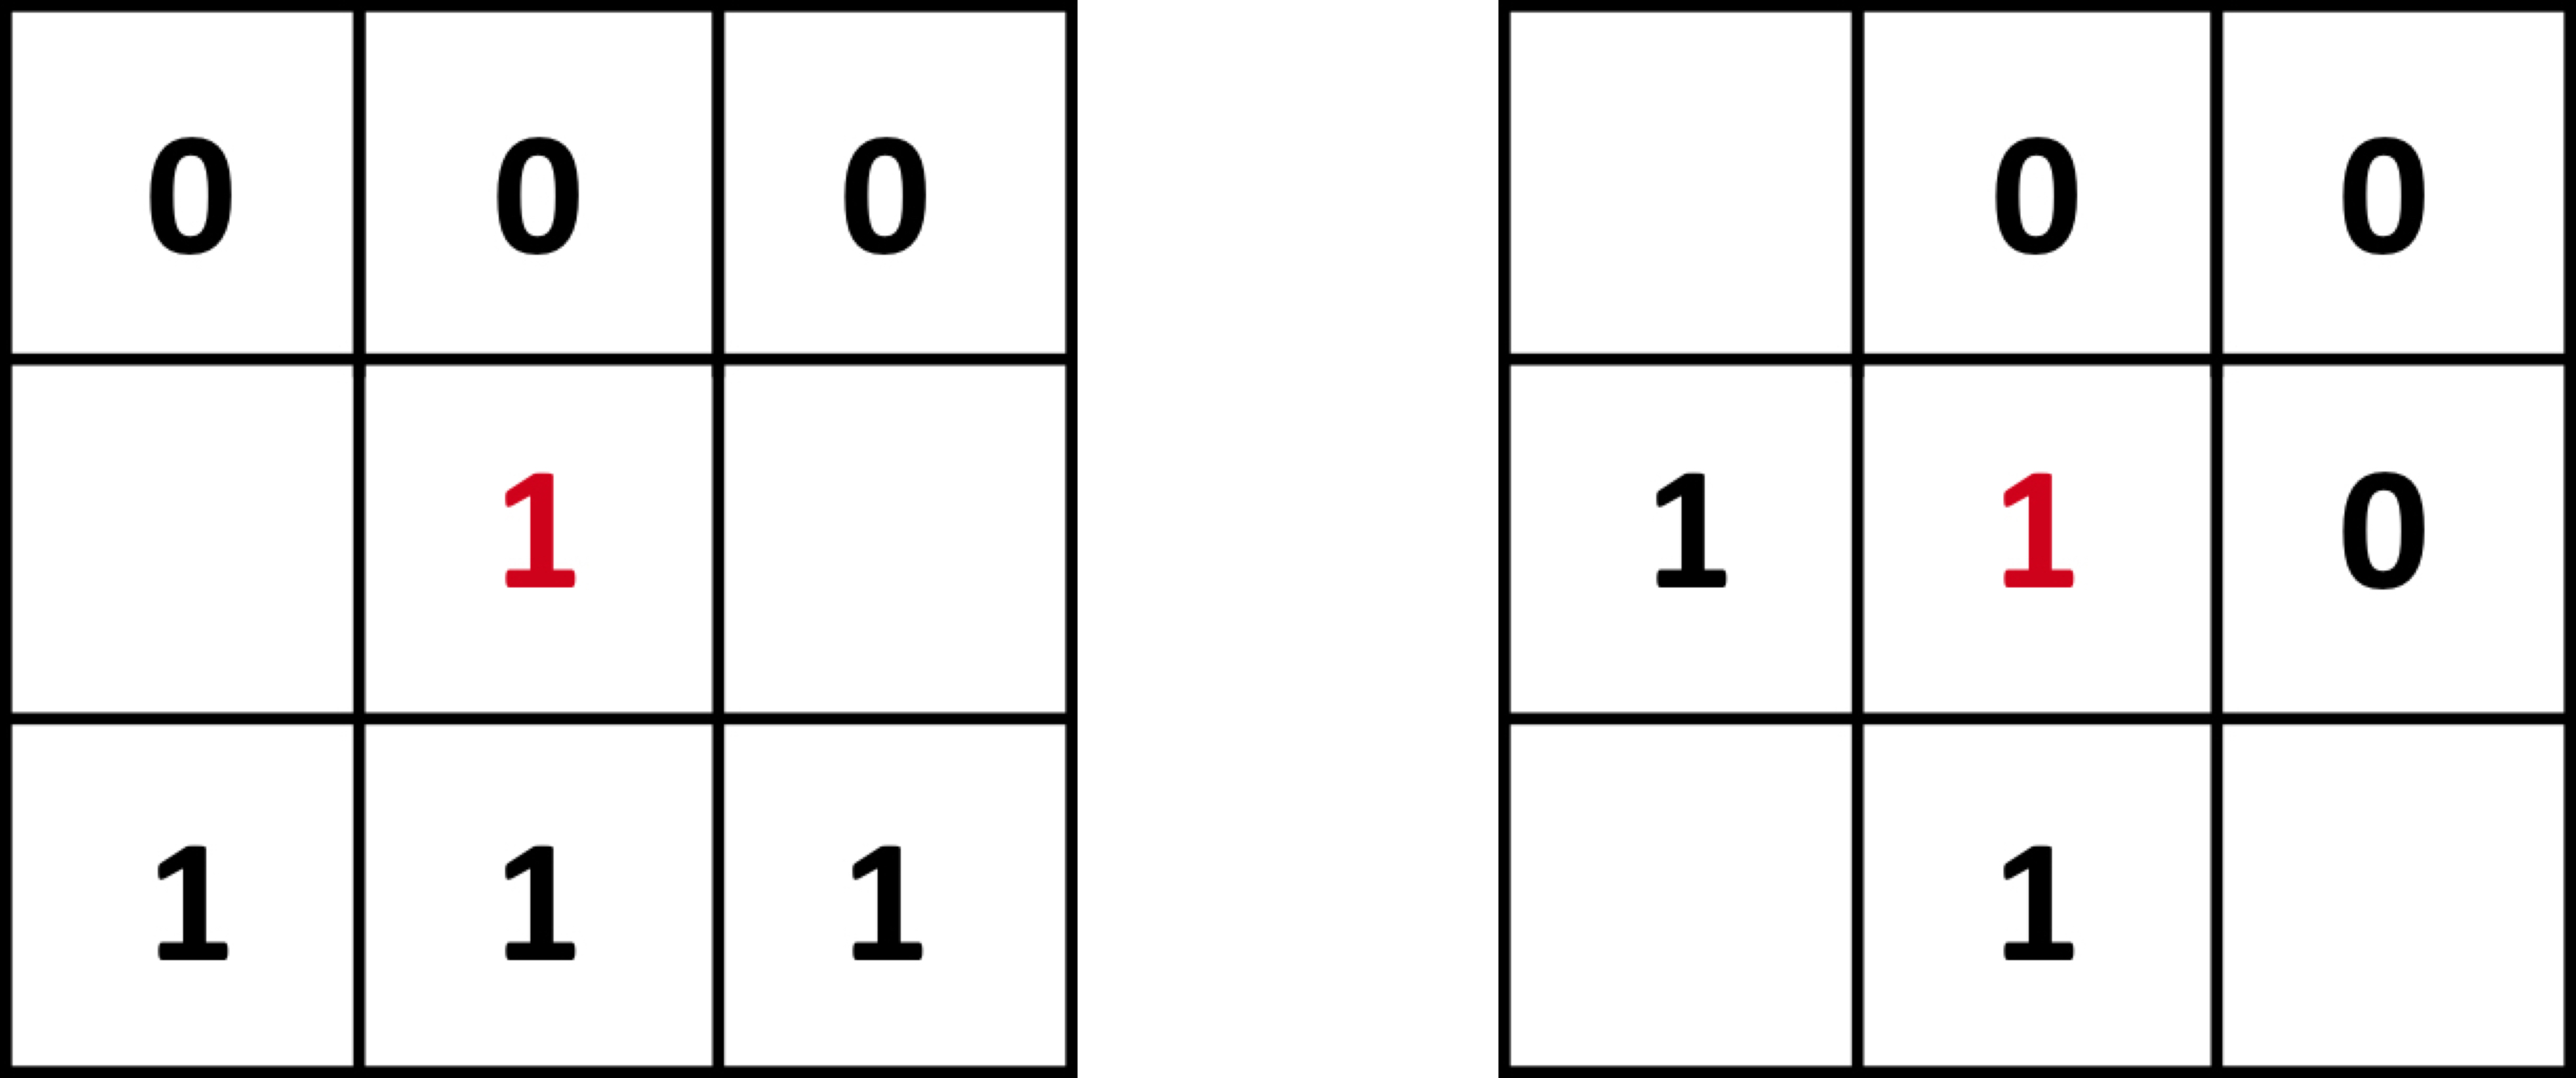
\includegraphics[width=10cm]{images/thinning_el.jpg}
    \caption{Strukturni elementi za stanjivanje}
    \label{fig:thinning_el}
\end{figure}

Navedeni algoritam nije pogodan za računalnu implementaciju što zbog kompliciranosti implementacije što zbog same brzine jer se praktički koristi osam strukturnih elemenata s kojima treba vršiti usporedbu. No Zhang i Suen su u svom radu \citep{Zhang-Suen}, davne 1984. predložili i opisali algoritam jednostavan za implementaciju na računalu. Princip ostaje isti, no umjesto osam strukturnih elemenata postoji samo jedan prikazan na slici \ref{fig:thinning_el_zhang}. Vrijednosti P na danom strukturnom elementu mogu poprimiti vrijednosti 0 ili 1, ovisno o tome je li slikovni element bijele ili crne boje, te se vrše izračunavanja u odnosu na susjedne slikovne elemente centralnom elementu, te unutar jedne iteracije postoje dvije pod-iteracije.

\begin{figure}[htb]
    \centering
    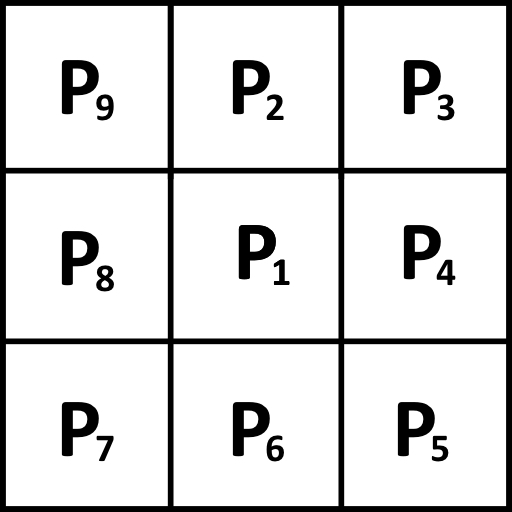
\includegraphics[width=4cm]{images/kernel.jpg}
    \caption{Zhang-Suenov strukturni element za stanjivanje}
    \label{fig:thinning_el_zhang}
\end{figure}

U prvoj pod-iteraciji, danim strukturnim elementom, briše se slikovni element na poziciji $P_1$ ukoliko su zadovoljeni sljedeći uvjeti:
\begin{gather} 
    2 \leq B(P_1) \leq 6, \\
    A(P_1) = 1, \\
    P_2\cdot P_4\cdot P_6 = 0 \  i\\ 
    P_4\cdot P_6\cdot P_8 = 0
\end{gather}
gdje je $A(P_1)$ broj '01' uzoraka u poretku $P_1, P_2, ...P_8, P_9$ i $B(P_1)$ broj crnih susjeda, to jest: 
\begin{gather} 
    B(P_1) = P_2 + P_3 + ... + P_8 + P_9.
\end{gather}
U drugoj pod-iteraciji mijenjanju se zadnja dva uvjeta u sljedeće:
\begin{gather} 
    P_2\cdot P_4\cdot P_8 = 0 \  i \\
    P_2\cdot P_6\cdot P_8 = 0,
\end{gather}
dok sve ostalo ostaje isto kao i u prvoj pod-iteraciji. Navedene iteracije se vrše naizmjence sve dok dana slika ne konvergira, to jest dok nakon zadnje iteracije više se ne obriše niti jedan slikovni element.

Na slici \ref{fig:thinning_good} prikazan je rad algoritma stanjivanja prema \emph{Zhang-Suenu}.
\begin{figure}[htb]
    \centering
    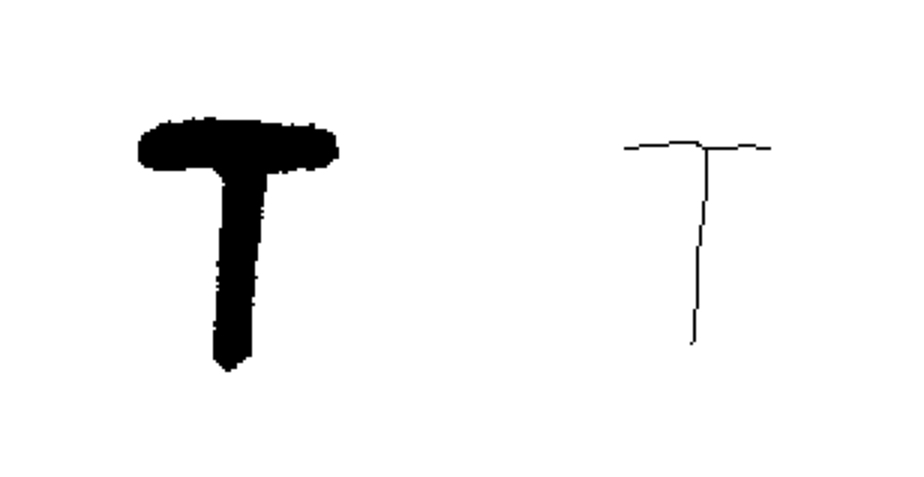
\includegraphics[width=8cm]{images/thinning_good.jpg}
    \caption{Stanjivanje prema \emph{Zhang-Suenu}}
    \label{fig:thinning_good}
\end{figure}

Na slici \ref{fig:thinning_bad} demonstriran je problem rada algoritma nad deformiranim objektom. Dakle, algoritam malu "rupicu" vidi kao pozadinu te oko nje gradi granice objekta, no tu u pomoć uskače dilatacija koja prikazanu nepravilnost ispuni.

\begin{figure}[htb]
    \centering
    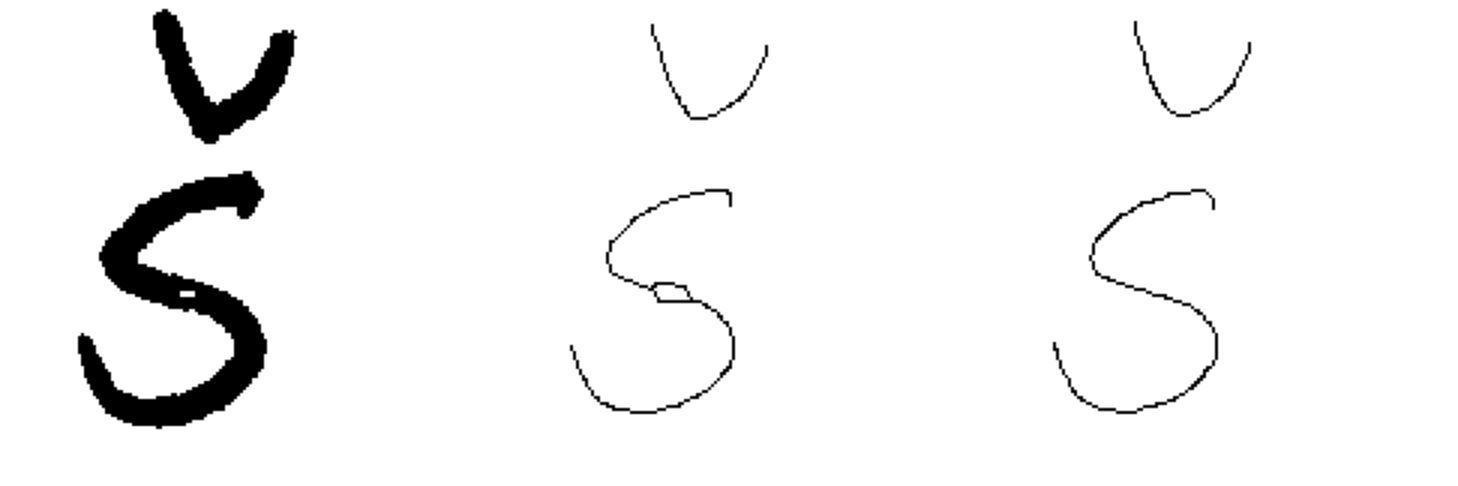
\includegraphics[width=12cm]{images/thinning_bad.jpg}
    \caption{Stanjivanje provedeno prije (srednja slika) i nakon (desna slika) dilatacije}
    \label{fig:thinning_bad}
\end{figure}

Implementacija iteracije prema \emph{Zhang-Suenu} u programskom jeziku \emph{Java} dana je sljedećim izvornim kodom.
\lstset{language=Java, tabsize=2}
\begin{lstlisting}
    private int[][] thinningIteration(Iteration iteration, int[][] inputImage) {
        int[][] marker = new int[width][height];
        for (int i = 1; i < width - 1; i++) {
            for (int j = 1; j < height - 1; j++) {
                int p2 = inputImage[i - 1][j];
                int p3 = inputImage[i - 1][j + 1];
                int p4 = inputImage[i][j + 1];
                int p5 = inputImage[i + 1][j + 1];
                int p6 = inputImage[i + 1][j];
                int p7 = inputImage[i + 1][j - 1];
                int p8 = inputImage[i][j - 1];
                int p9 = inputImage[i - 1][j - 1];

                int c1 = p2 == 0 && p3 == 1 ? 1 : 0;
                int c2 = p3 == 0 && p4 == 1 ? 1 : 0;
                int c3 = p4 == 0 && p5 == 1 ? 1 : 0;
                int c4 = p5 == 0 && p6 == 1 ? 1 : 0;
                int c5 = p6 == 0 && p7 == 1 ? 1 : 0;
                int c6 = p7 == 0 && p8 == 1 ? 1 : 0;
                int c7 = p8 == 0 && p9 == 1 ? 1 : 0;
                int c8 = p9 == 0 && p2 == 1 ? 1 : 0;

                int A = c1 + c2 + c3 + c4 + c5 + c6 + c7 + c8;
                int B = p2 + p3 + p4 + p5 + p6 + p7 + p8 + p9;
                int m1 = 0; int m2 = 0;
                switch (iteration) {
                    case ITERATION_FIRST:
                        m1 = (p2 * p4 * p6);
                        m2 = (p4 * p6 * p8);
                        break;
                    case ITERATION_SECOND:
                        m1 = (p2 * p4 * p8);
                        m2 = (p2 * p6 * p8);
                        break;
                }
                if (A == 1 && (B > 1 && B < 7) && m1 == 0 && m2==0)
                    marker[i][j] = 1;
            }
        }
        return outputImageFromMarker(inputImage, marker);
    }
\end{lstlisting}

\section{Segmentacija i skaliranje slova}

Posljednji korak pri obradi danog skupa podataka rukom pisanih slova je segmentacija i skaliranje pojedinog binarnog slova. Razlog tomu je postizanje invarijantnost pojedinog slova na dimenzije, što bi, ukoliko nije provedeno, kasnije predstavljalo problem prilikom klasifikacije pojedinog slova ukoliko su ista slova različitih dimenzija.

Prvi korak je segmentacija slova. Kako su već sva slova izdvojena s obrasca i pretvorena u crno-bijelu sliku algoritam je vrlo jednostavan. Dakle, potrebno je pronaći najmanji pravokutnik koji omeđuje slovo. Kako je slika crno-bijela, algoritam se svodi na pretraživanje \emph{x} vrijednosti najbližeg i najdaljeg crnog slikovnog elementa po visini slike, te \emph{y} vrijednosti za najbližeg i najdaljeg crnog slikovnog elementa po dužini slike, kako je prikazano na slici \ref{fig:crop_example}.
\begin{figure}[htb]
    \centering
    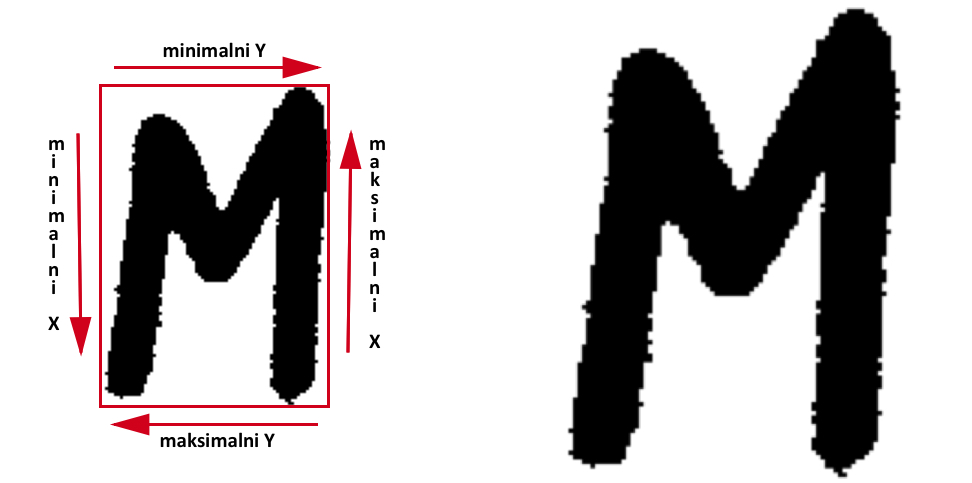
\includegraphics[width=12cm]{images/crop_example.jpg}
    \caption{Segmentacija slova}
    \label{fig:crop_example}
\end{figure}

Nakon segmentacije slijedi skaliranje izdvojenog slova. Za potrebe ovog rada sva izdvojena slova su skalirana na kvadratne dimenzije $30 \times 30$. Kod skaliranja slike postoji više načina i pristupa, no neki od poznatijih su bilinearna i bikubična interpolacija koje pokušavaju sačuvati glatkost slike. No kako je slika slova binarna, to jest crno-bijela, bilinearna ili bikubična interpolacija bi napravila više štete nego koristi jer bi aproksimacijom slikovnog elementa rezultat mogao biti iz područja sive boje, dakle više ne bi bila binarna slika te bi opet trebalo obaviti binarizaciju. Stoga je za potrebe ovog rada korištena metoda najbližeg susjeda.

\begin{figure}[htb]
    \centering
    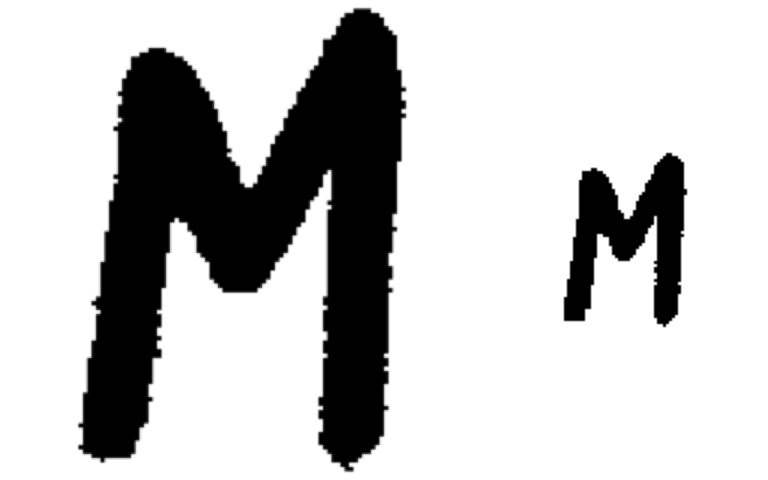
\includegraphics[width=8cm]{images/resize_example.jpg}
    \caption{Skaliranje slova}
    \label{fig:resize_example}
\end{figure}

Prilikom uvećavanja slike u slici nastaju praznine, kod metode najbližeg susjeda, kako joj i ime kaže, uzima se vrijednost najbližeg slikovnog elementa te se postavlja na trenutnu prazninu. Nema interpolacije više vrijednosti, pa će binarna slika ostati binarna. Kod smanjivanja slike princip je isti, samo što umjesto popunjavanja praznina slijedi izuzimanje slikovnog elementa te se uzima samo onaj najbliži. Prikaz rada algoritma vidljiv je na slici \ref{fig:resize_example}. Bitno je napomenuti da je metoda najbližeg susjeda najjednostavnija te da bi se pri obradi slike u boji trebala izbjegavati i koristiti neku od već gore spomenutih.

Za potrebe ovog rada segmentacija i skaliranje slova se zbivala nakon binarizacije slike, te se nakon toga po potrebi odvijala dilatacija, pa zatim stanjivanje prednjeg plana. Implementacija skaliranja slike metodom najbližeg susjeda u programskom jeziku \emph{Java} dana je sljedećim izvornim kodom.
\lstset{language=Java, tabsize=2}
\begin{lstlisting}
    public BufferedImage applyFilter(BufferedImage sourceImage, int newWidth, int newHeight) {
        int width = sourceImage.getWidth();
        int height = sourceImage.getHeight();
        BufferedImage scaledImage = new BufferedImage(
                newWidth, newHeight, sourceImage.getType());
        float xRatio = width / (float) newWidth;
        float yRatio = height / (float) newHeight;
        int x, y;
        for (int i = 0; i < newWidth; i++) {
            for (int j = 0; j < newHeight; j++) {
                x = (int) Math.floor(i * xRatio);
                y = (int) Math.floor(j * yRatio);
                scaledImage.setRGB(i, j, sourceImage.getRGB(x, y));
            }
        }
        return scaledImage;
    }
\end{lstlisting}

\chapter{Klasifikacija}
Nakon što su obrasci skenirani, obrađeni, slova segmentirana i pripremljena za daljnju obradu na red dolazi određivanje razreda, odnosno slova abecede, pojedinoj slici slova, to jest klasifikacija. Za klasifikaciju prikupljenoga skupa podataka korištena je slojevita potpuno povezana unaprijedna umjetna neuronska mreža koja je učena algoritmom propagacije pogreške unatrag, točnije jednom varijantom navedenoga algoritma koja koristi inerciju kako bi se pospješilo i ubrzalo učenje.

\section{Motivacija i povijesni razvoj}

U današnje doba, uz nevjerojatne brojke o količini memorije, brzine procesora i razno raznih tehničkih detalja koji se iznose prilikom predstavljanja super-računala te o količini podataka koje obrađuju, ta brojka još uvijek nije ni blizu onoj brojci podataka koja se u svakom trenutku obrađuju u mozgu i živčanom sustavu živih bića. Ponukani tom idejom, Warren McCulloch i Walter Pitts u svom su radu \emph{A logical calculus of the ideas immanent in nervous activity} još 40-ih godina prošlog stoljeća predstavili model umjetnog neurona \engl{TLU perceptron} i pokazali da se njime mogu računati logičke funkcije I, ILI i NE, iz čega slijedi da se kombinacijom više tih neurona u neuronsku mrežu može dobiti proizvoljno kompleksna Booleova funkcija \citep{nenr}.

Nekoliko godina nakon navedenoga dvojca, britanski biolog Donald Hebb je u svojoj knjizi \emph{The Organization of Behavior} izjavio da \emph{učiti znači mijenjati jakosti veza između neurona}, što je Frank Rosenblatt 1957. godine iskoristio kao temelj za ostvarivanje algoritma učenja TLU perceptrona, što je bio velik uspjeh jer je uspio pokazati da se određeni problemi mogu rješavati učenjem, a ne samo konstrukcijom, kako su to Pitts i McCulloch pokazali.

Sam razvoj neuronskih mreža počeo je kao pokušaj da se objasni inteligentno ponašanje ljudi i životinja i to putem simbolističkog pristupa koji je kao cilj imao znanje iz neke domene obuhvatiti skupom atomičkih semantičkih objekata (simbola) i zatim činit niz manipulacija tih simbola pomoću algoritamskih pravila, no daljnjim istraživanjem mozga pokazano je da je takav pristup neutemeljen i nemoguć prilikom oponašanja inteligentnih bića jer su mozak i živčani sustav sastavljeni od velikog broja procesnih elemenata, odnosno neurona, koji obrađuju velike količine informacija paralelno, što je temelj pristupa koji je danas poznat pod nazivom konektivizam.

\section{Osnovni model umjetnog neurona}
Neuron, kao osnovna građevna jedinica živčanog sustava, prikazan je na slici \ref{fig:biological_neuron}. Ukratko, svaki neuron čini \emph{tijelo stanice} koje sadrži jezgru. Na rubovima tijela stanice nalaze se \emph{dendirit}, koji služe kao poveznica s ostalim neuronima te dovode impuls do \emph{tijela stanice}. Iz neurona kao izlaz prema ostalim neuronima služi produžetak nazvan \emph{akson}. U tijelu stanice vlada određeni električni potencijal, te promjenom tog potencijala nastaje elektrokemijski impuls koji se dalje širi aksonom koji je povezan s dendritima do 10000 drugih neurona. Prijenosom impulsa od neurona do neurona zapravo se odvija proces prijenos informacija koji je određen jakostima sinaptičkih veza između pojedinih neurona.
\begin{figure}[htb]
    \centering
    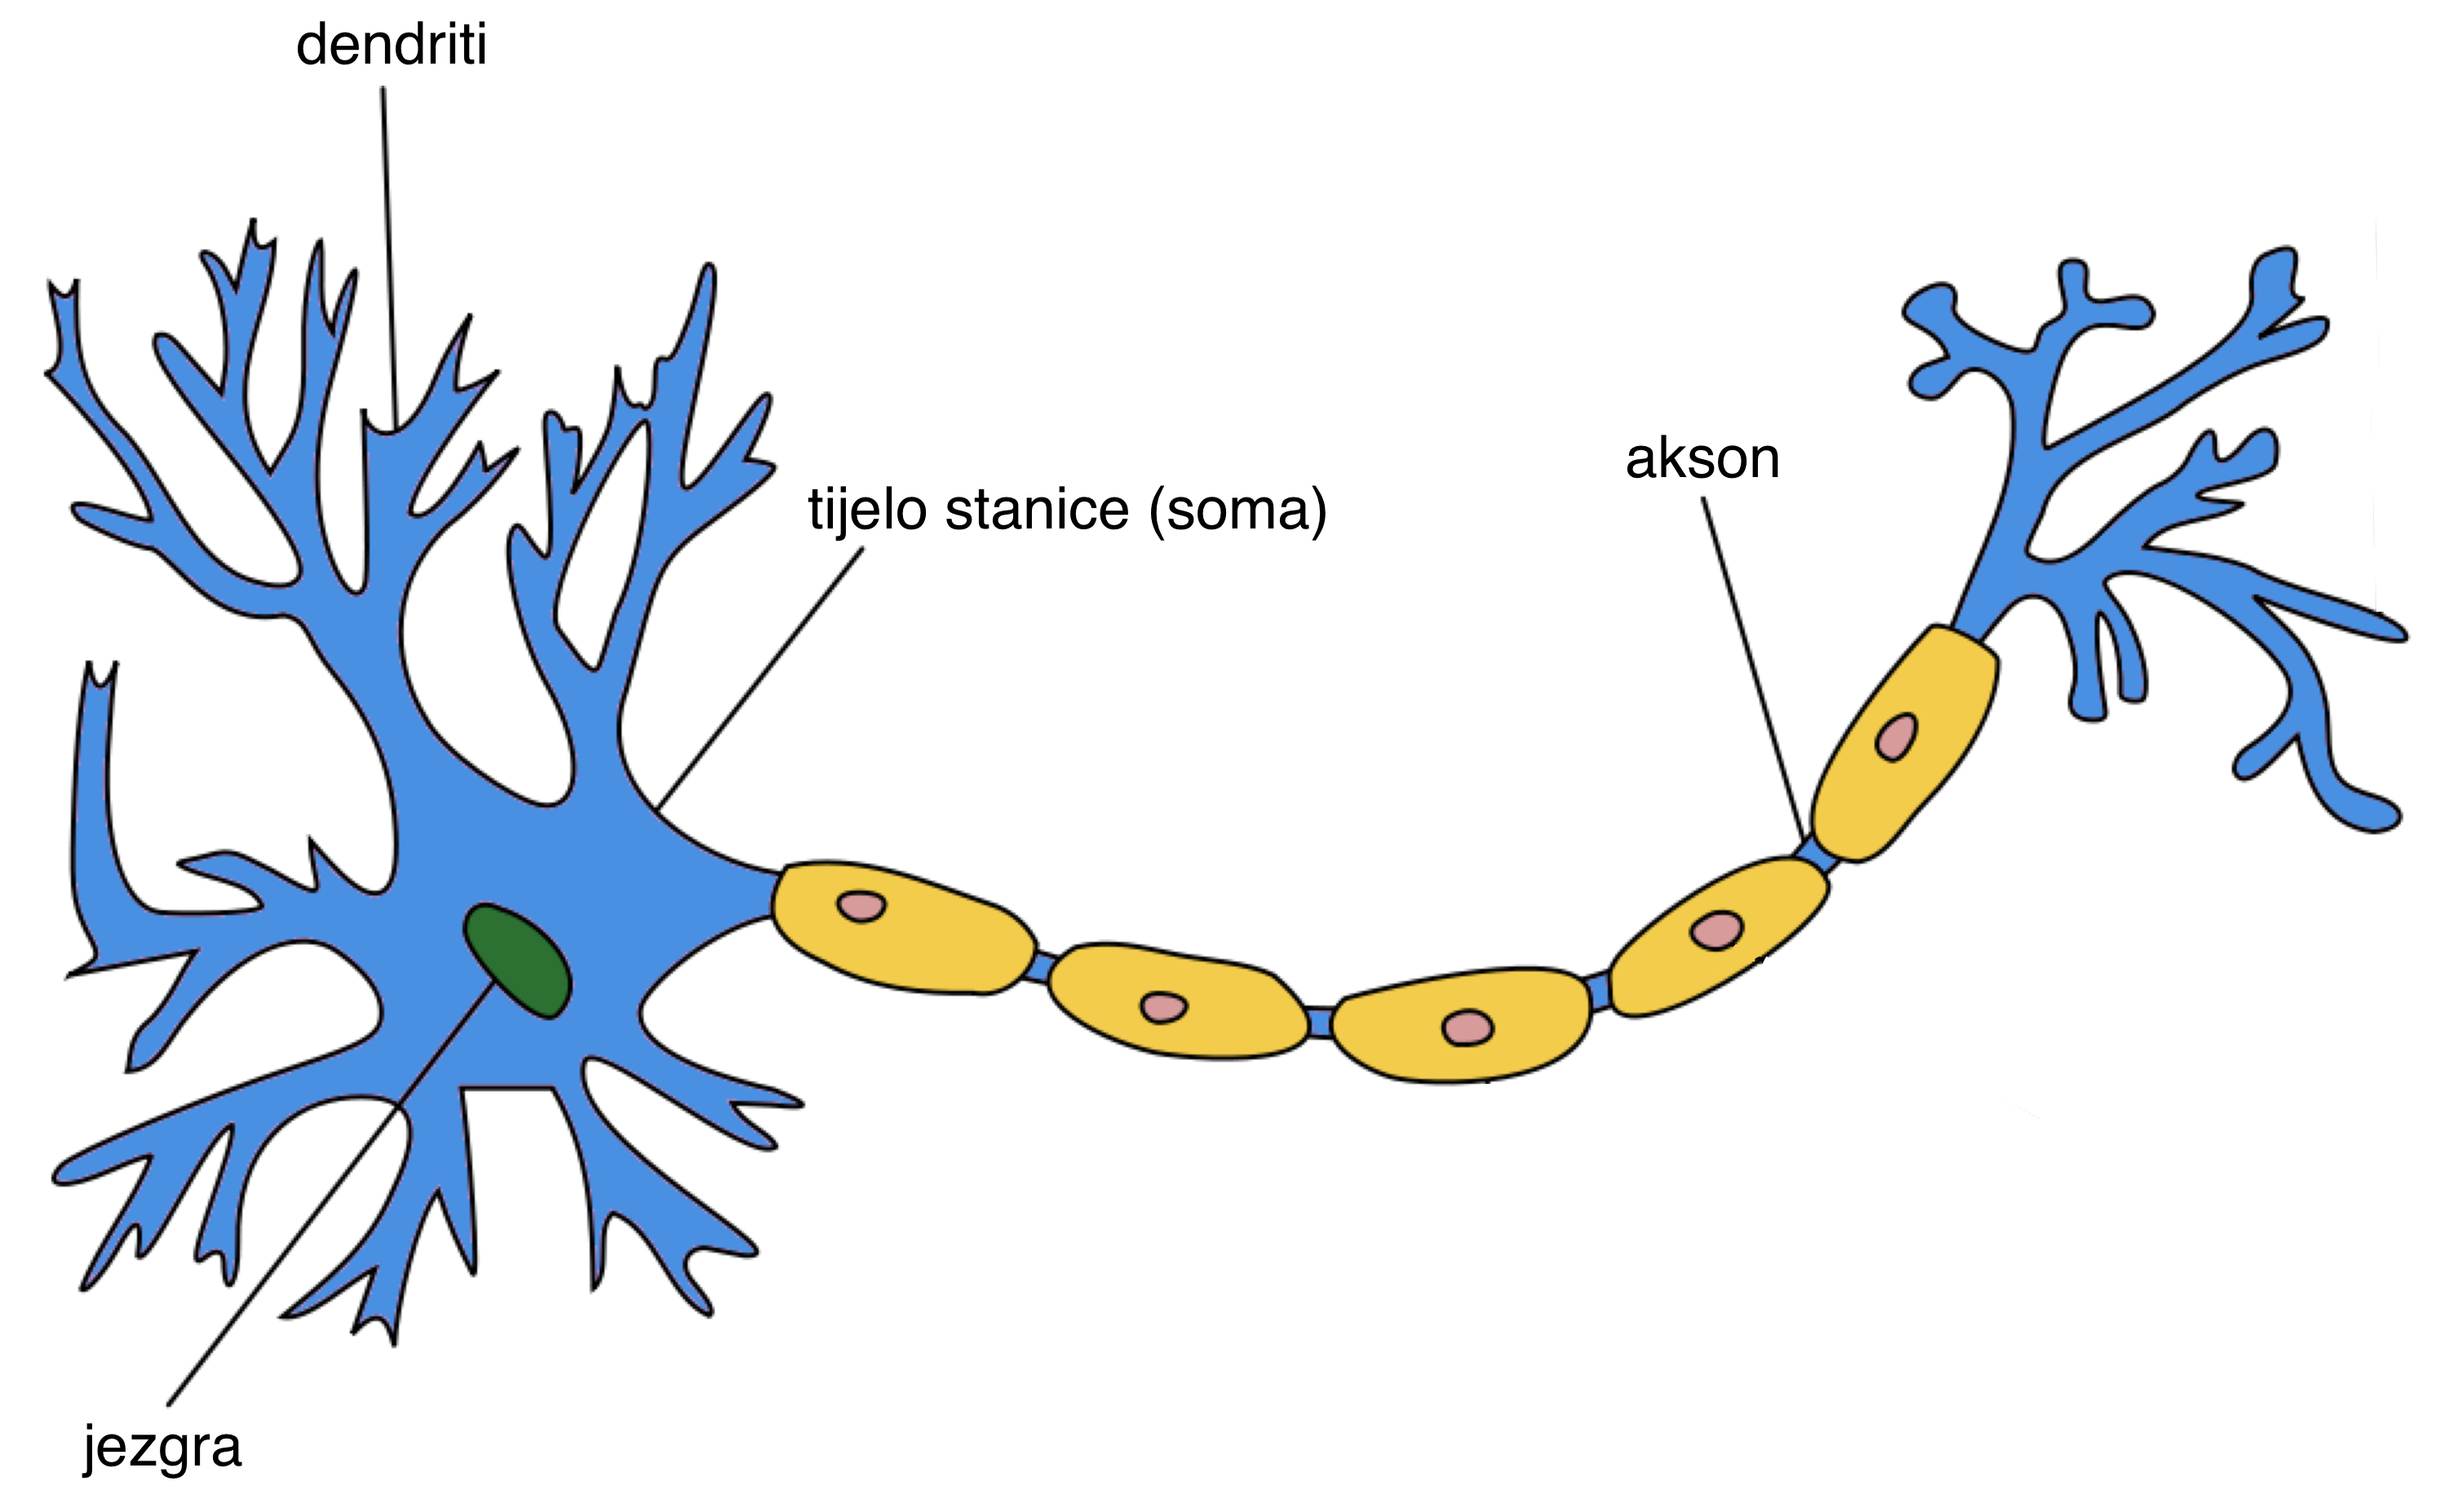
\includegraphics[width=14cm]{images/biological_neuron.jpg}
    \caption{Biološki neuron, preuzeto iz \citep{wikiNeuron}}
    \label{fig:biological_neuron}
\end{figure}

Kako je već spomenuto Warren McCulloch i Walter Pitts su 1943. godine povukli analogiju s biološkim neuronom te definirali model umjetnog neurona prikazanog na slici \ref{fig:neuron_model}. Umjetni model neurona se sastoji od ulaza $x_1, x_2, ..., x_n$ koji predstavljaju dendrite, preko kojih neuron prima pobudu od drugih neurona ili vanjskog svijeta. Utjecaj pojedinog ulaza na neuron definiran je težinama $w_1, w_2, ..., w_n$. Djelovanje pojedinog ulaza, to jest u kojoj mjeri pobuđuje neuron, definirano je umnoškom $w_1 \cdot x_1$.
\begin{figure}[htb]
    \centering
    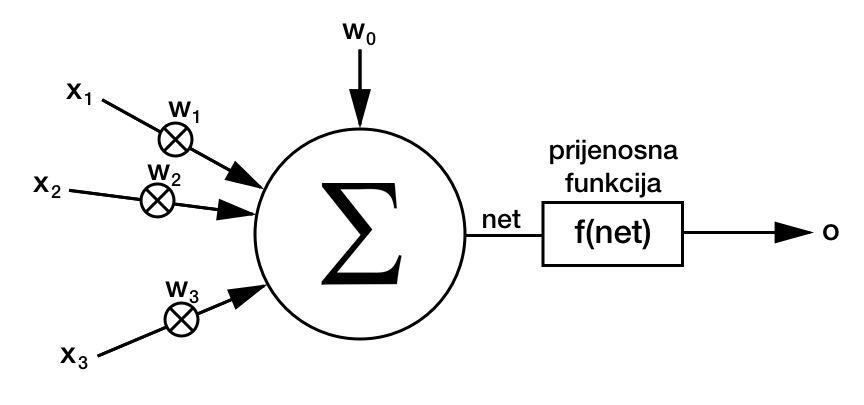
\includegraphics[width=14cm]{images/neuron_model.png}
    \caption{Osnovni model umjetnog neuron}
    \label{fig:neuron_model}
\end{figure}
Tijelo neurona se ponaša kao zbrajalo te na svom izlazu \emph{net} daje ukupnu pobudu. Ukupna pobuda neurona definirana je izrazom: $$net = \sum_{i=0}^{n} w_i \cdot x_i$$ gdje $x_0$ predstavlja fiktivni ulaz čija je vrijednost uvijek 1 (tako je prikazano radi ljepšeg zapisa), te težina $w_0$ predstavlja prag paljenja neurona.

Prijenosna funkcija \engl{transfer function} modelira ponašanje aksona te određuje konačni izlaz neurona u ovisnosti o ukupnoj pobudi. Prilikom modeliranja TLU perceptrona, McCulloch i Pitts su koristili prijenosnu funkciju skoka prikazanu na slici \ref{fig:step} te definiranu izrazom:
\[
  f(net) = \left\{\def\arraystretch{1.2}%
  \begin{array}{@{}c@{\quad}l@{}}
    0, & \text{$net \leq 0$} \\
    1, & \text{inače.}\\
  \end{array}\right.
\]
Bitno je napomenuti da se od neurona koji koriste linearne prijenosne funkcije ne mogu graditi složene neuronske mreže, jer se od linearnih elemenata ne može dobiti ništa složenije, to jest cijela se mreža opet pretvara u linearni element.
\begin{figure}[htb]
    \centering
    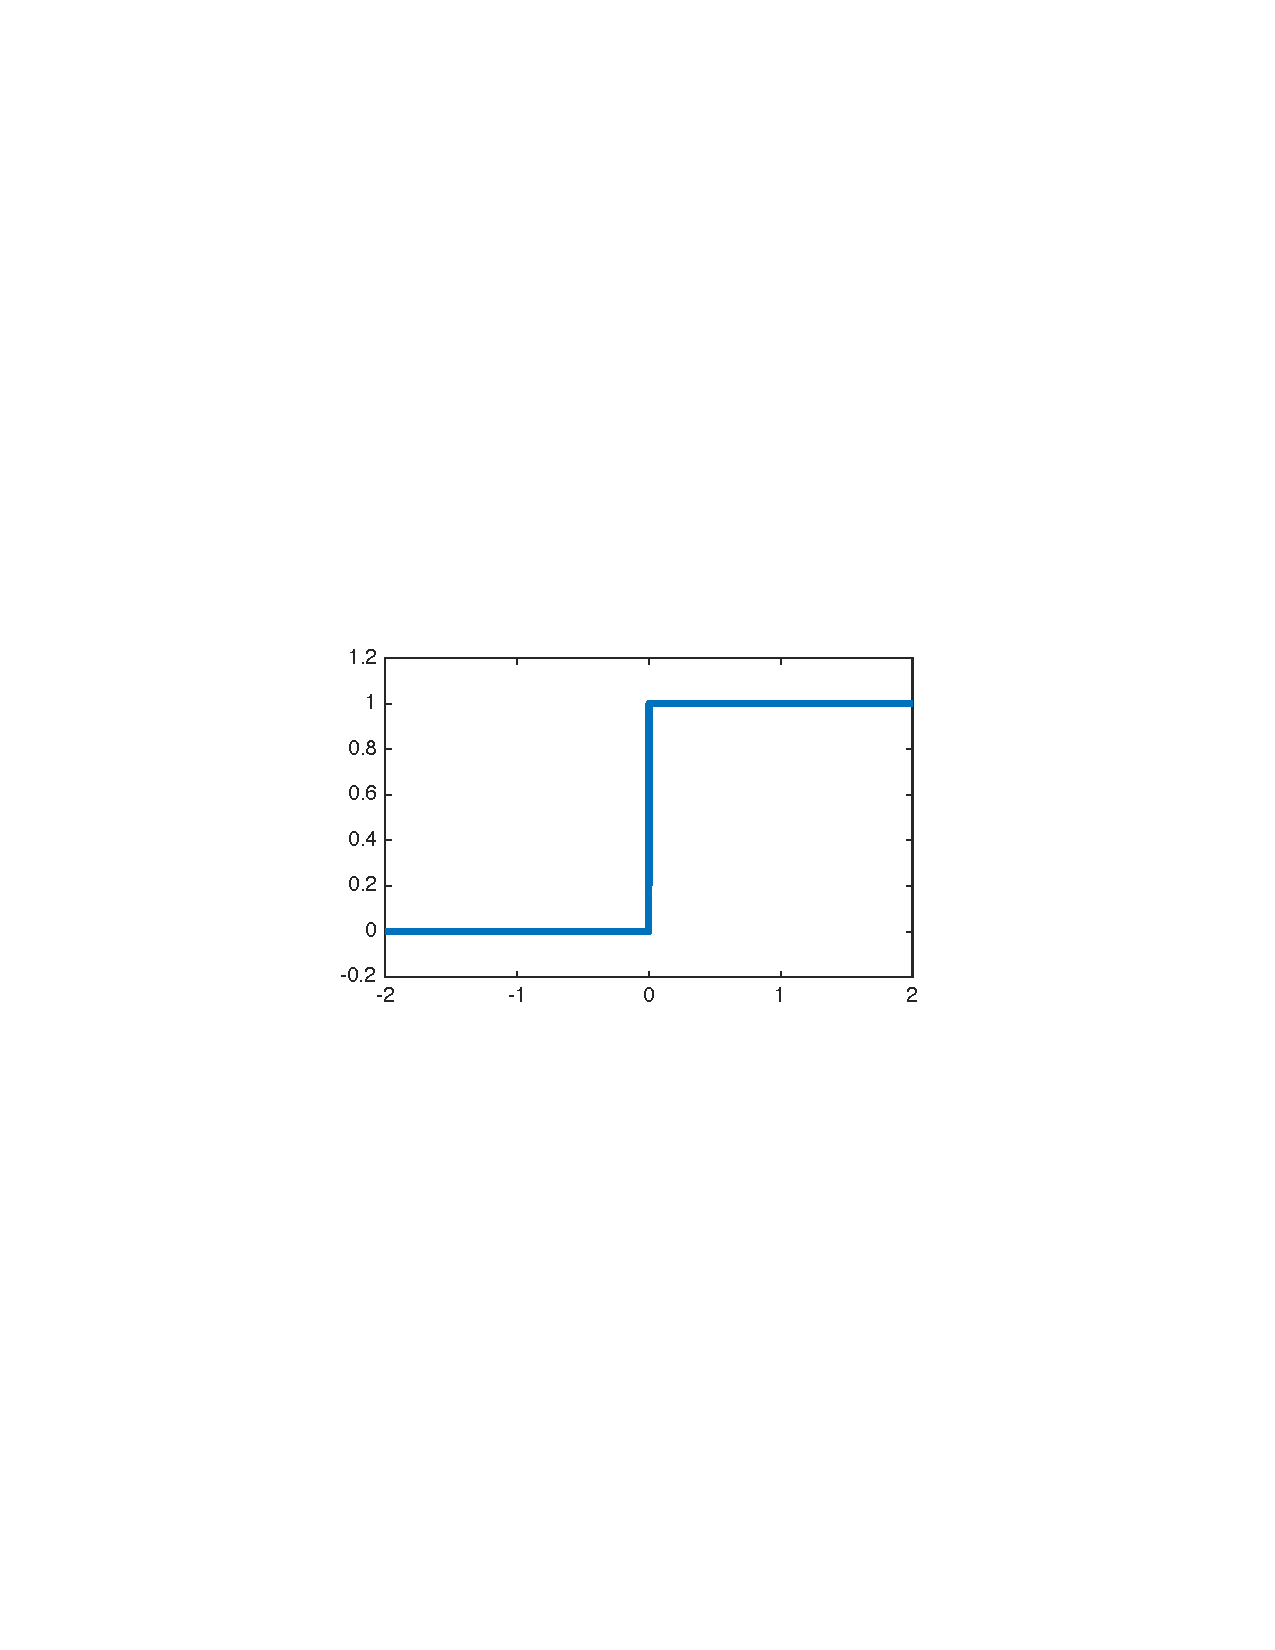
\includegraphics[width=10cm]{images/step.pdf}
    \caption{Funkcija skoka}
    \label{fig:step}
\end{figure}

U početku je bio velik problem definiranje algoritma učenja složenijih neuronskih mreža. No riješenje navedenoga problema se pojavilo u obliku algoritma propagacije pogreške unatrag uvođenjem derivabilnih prijenosnih funkcija. Najpoznatiji predstavnik te skupine prijenosnih funkcija je sigmoidalna (logistička) funkcija prikazana na slici \ref{fig:sigmoidal}, te definirana sljedećim izrazom: $$f(net) = \frac{1}{1+e^{-net}}$$
\begin{figure}[htb]
    \centering
    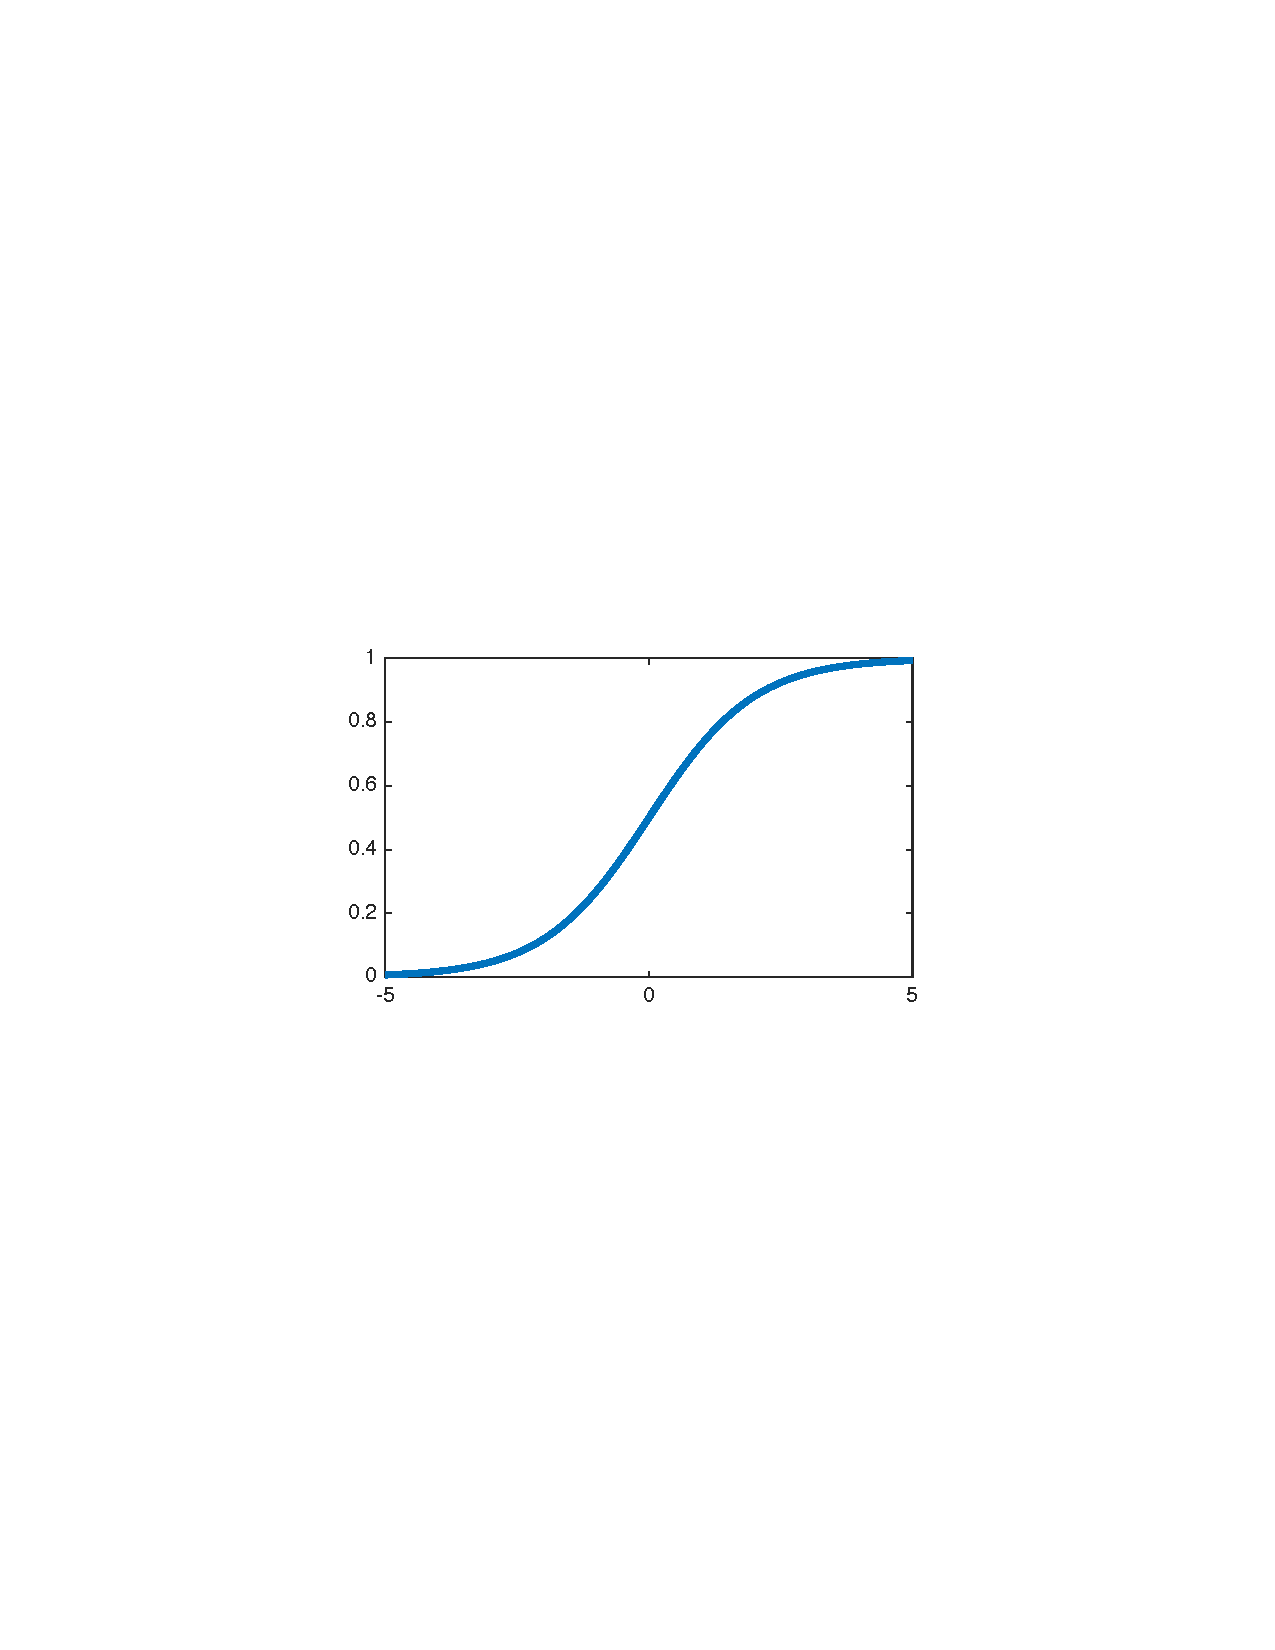
\includegraphics[width=10cm]{images/sigmoidal.pdf}
    \caption{Sigmoidalna (logistička) funkcija}
    \label{fig:sigmoidal}
\end{figure}

Za potrebe ovog rada prilikom učenja neuronske mreže korišten je algoritam propagacije pogreške unatrag te navedena sigmoidalna (logistička) prijenosna funkcija. Navedeni algoritam učenja bit će pobliže opisan u poglavlju o učenju neuronske mreže, no prije toga slijedi kratak osvrt na osnovni model neuronske mreže.

\section{Osnovni model neuronske mreže}

Skup jednostavnih procesnih jedinica, odnosno umjetnih neurona, koji su povezani u paralelne strukture različitih arhitektura naziva se umjetna neuronska mreža. Primjer jedne takve umjetne neuronske mreže prikazan je na slici \ref{fig:neural_net}.
\begin{figure}[htb]
    \centering
    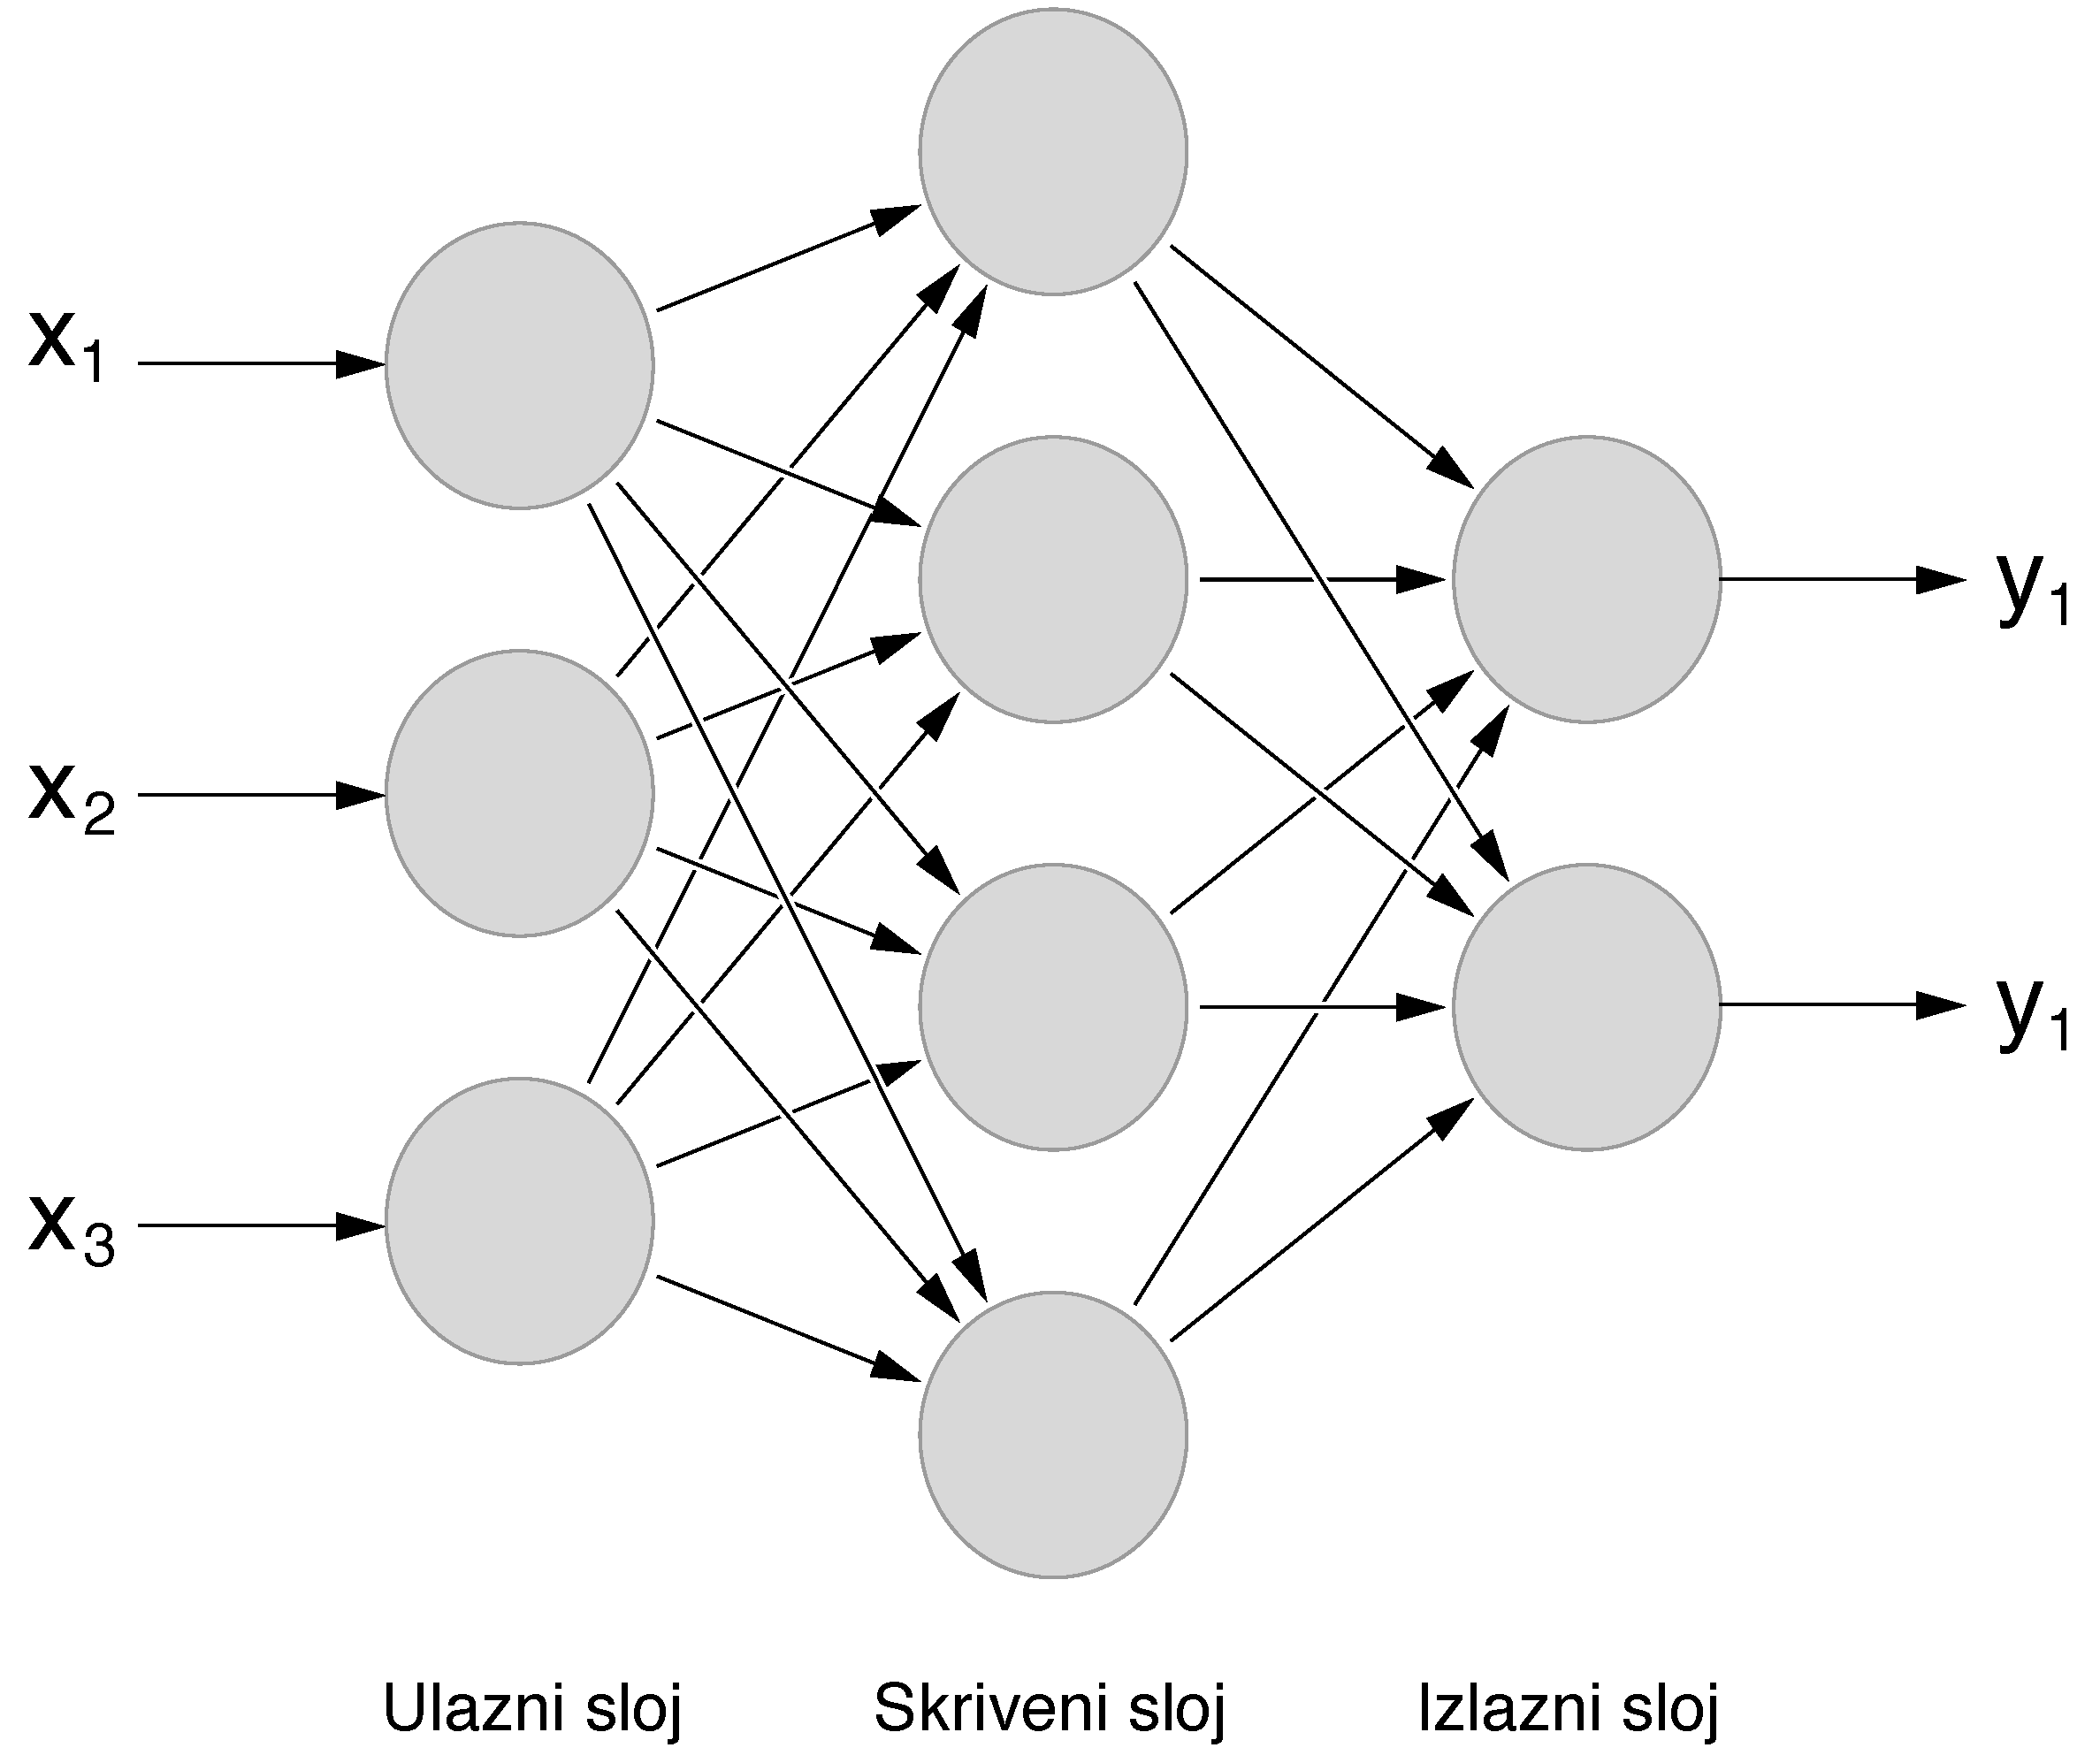
\includegraphics[width=12cm]{images/neural_net.pdf}
    \caption{Primjer potpuno povezane unaprijedne neuronske mreže}
    \label{fig:neural_net}
\end{figure}

S lijeve strane neuronske mreže nalaze se ulazni neuroni. Na njih se dovodi informacija koju je potrebno obraditi te kao takvi ne obavljaju nikakvu obradu već služe samo za prosljeđivanje ulaznih podataka na iduće slojeve mreže. Idući sloj je skriveni sloj, na slici je prikazan samo jedan no unutrašnjost mreže može biti sastavljena od više skrivenih slojeva. Unutar skrivenih slojeva se zbiva obrada informacija. Zadnji sloj, na slici krajnje desni, je izlazni sloj koji nakon obrade podataka dostavlja konačne rezultate okolini.

Arhitektura mreže određena je s više parametara. Jedan od njih je i broj skrivenih slojeva te broj neurona u pojedinom sloju. Mreža prikazana na slici \ref{fig:neural_net} je strukture \mbox{$3 \times 4 \times 2$} (pojedini sloj je odvojen znakom $\times$, te brojka predstavlja broj neurona u pojedinom sloju). Također, povezanost među neuronima određuje arhitekturu mreže. Mreža iz primjera je potpuno povezana slojevita, jer su neuroni iz sloja $n$ povezani sa svim neuronima iz sloja $n+1$, gledano s lijeva na desno. Prikazana mreža je među ostalim i unaprijedna mreža jer je smjer poveznica pojedinog sloja u smjeru s lijeva na desno, to jest iz smjera $n$ prema $n+1$. Mreža može biti i ciklička, gdje su primjerice neuroni pojedinog sloja povezani u oba pravca.

Za potrebe ovog rada korištena je potpuno povezana unaprijedna slojevita neuronska mreža u ponešto drugačijem broju neurona i skrivenih slojeva. U literaturi se takva mreža često navodi pod imenom višeslojni perceptron \engl{multilayer perceptron}.

\section{Učenje neuronske mreže}

Rad s umjetnim neuronskim mrežama se može podijeliti u dvije faze: prvu fazu ili fazu učenja \engl{training, learning} te drugu fazu ili fazu iskorištavanja kad se naučena neuronska mreža koristi za obradu podataka.

Prilikom faze učenja neuronskoj mreži se na ulaze dovode uzorci iz skupa uzoraka za učenje i kako je već ranije spomenuto da mijenjanje jakosti veza predstavlja učenje tako se i neuronskoj mreži mijenjaju jakosti veza, to jest težine, između međusobno povezanih neurona. Težine se mogu podešavati prilikom predočavanja svakog uzorka što se naziva pojedinačno učenje \engl{on-line learning} ili tek nakon što se mreži predoče svi uzorci iz skupa uzoraka što se naziva grupno učenje \engl{batch learning}. Predočavanje jednog uzorka neuronskoj mreži se naziva \emph{iteracija}, a predočavanje čitavog skupa uzoraka za učenje \emph{epoha}.

Postoji još jedna podjela načina učenja kod neuronskih mreža. Postoji nadzirano učenje \engl{supervised learning} ili učenje s učiteljem gdje se mreži predočavaju uzorci oblika $f(ulaz, zeljeni\ izlaz)$, a zadaća je mreže naučiti ispravno klasificirati pojedini uzorak. Kod učenja bez učitelja \engl{unsupervised learning}, uzorci koje dobiva neuronska mreža su oblika $\{(ulaz), ...,(ulaz)\}$ te mreža tada obavlja grupiranje podataka u pojedine razrede. Postoji još i podržano učenje \engl{reinforcement learning} gdje se mreža koristi kao model za aproksimaciju Q-vrijednosti stanja i akcija.

Prilikom učenja neuronske mreže cilj je postići da mreža dobro generalizira podatke iz domene koji su predočeni skupom za učenje. No skup za učenje, to jest bilo koji skup ulaznih podataka, sadrži određenu količinu šuma. Ukoliko se mreža krene prilagođavati prisutnom šumu u skupu podataka za učenje dolazi do pretreniranosti mreže i samim time gubi sposobnost generalizacije. Stoga, od iznimne je važnosti pratiti učenje mreže i onog trenutka kad se počne prilagođavati prisutnom šumu u podacima, to jest počne gubiti sposobnost generalizacije, zaustaviti učenje mreže.

Iz tog razloga, dostupni skup podataka se dijeli na tri podskupa: skup za učenje \engl{training set}, skup za provjeru \engl{validation set} te skup za testiranje \engl{testing set}. Mreža se uči predočavanjem podataka iz skupa za učenje. Učenje takve mreže se povremeno provjerava skupom za provjeru, primjerice nakon svake epohe. Bitno je napomenuti da prilikom te provjere mreži nije dopušteno da se prilagođava podacima iz skupa za provjeru. U početku učenja mreže ukupna greška kod prepoznavanja skupa za učenje i skupa za provjeru će padati, kako je i prikazano na slici \ref{fig:learning_curve}. No u jednom trenutku će se mreža početi prilagođavati šumu u skupu podatak za učenje i u tom trenutku ukupna greška nad skupom za provjeru početi rasti dok će nad skupom za učenje greška nastaviti padati, i zapravo u tom je trenutku potrebno zaustaviti učenje.
\begin{figure}[htb]
    \centering
    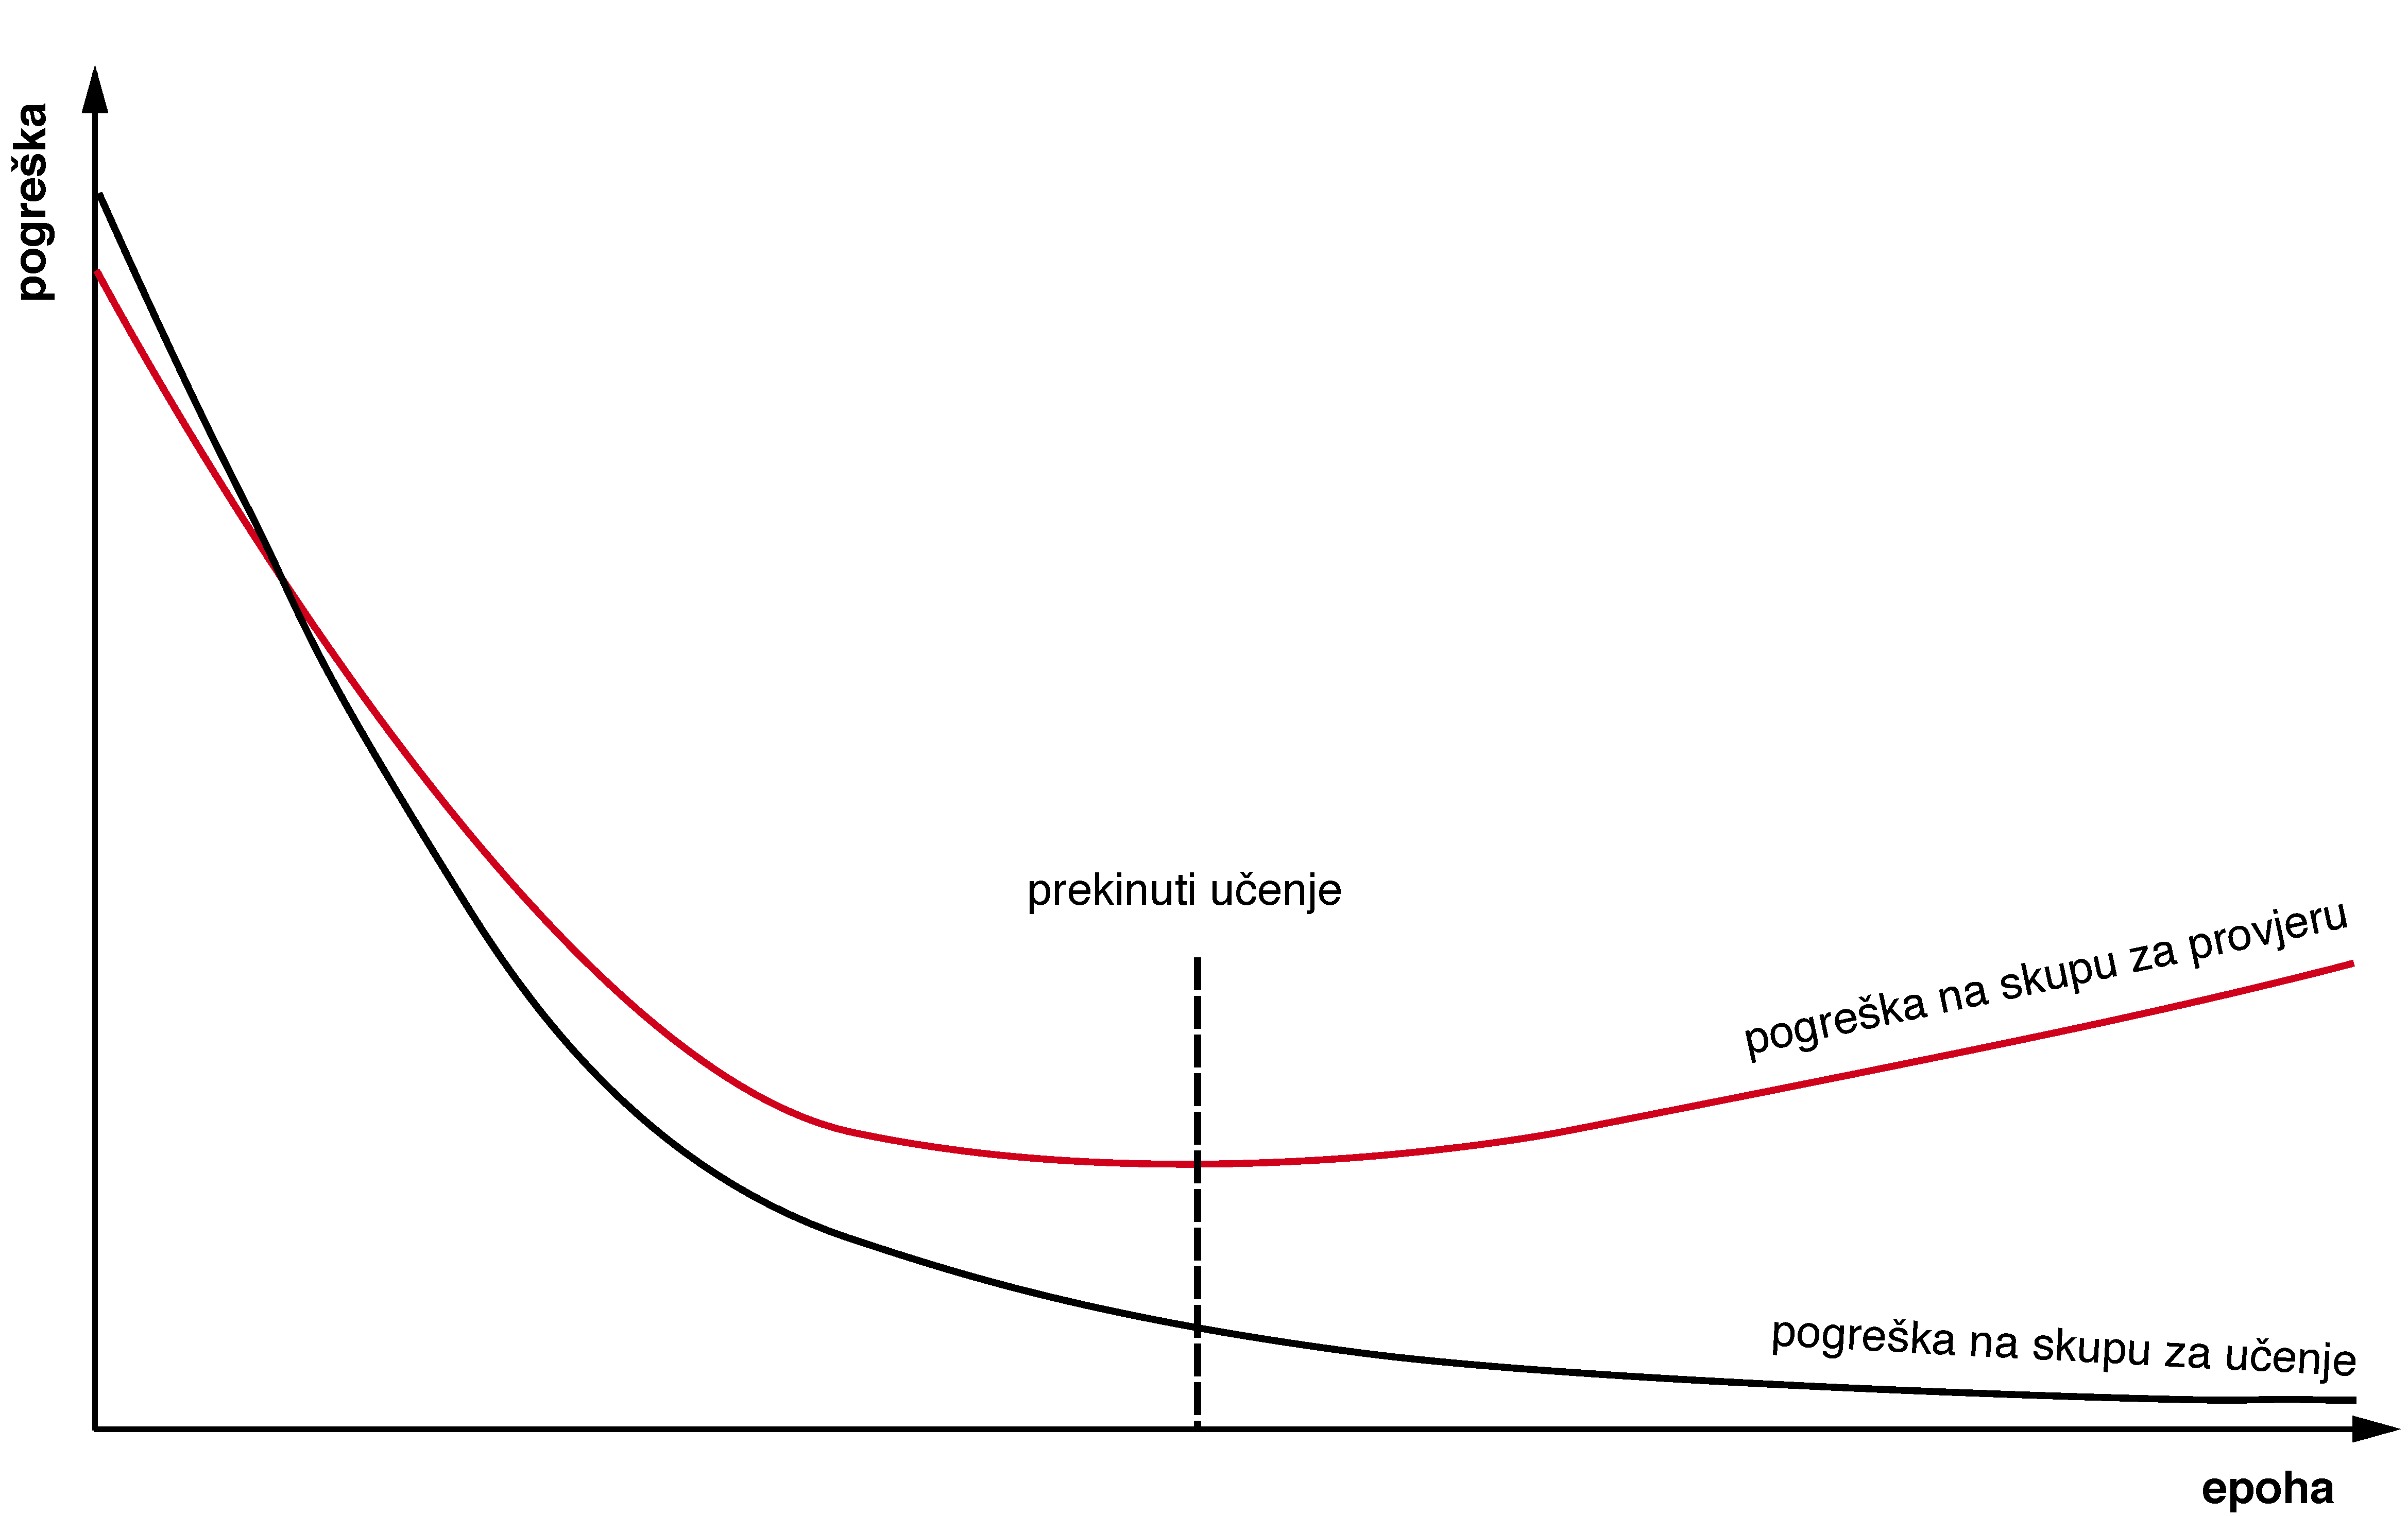
\includegraphics[width=14cm]{images/learning_curve.pdf}
    \caption{Pogreška prilikom učenja neuronske mreže}
    \label{fig:learning_curve}
\end{figure}

Nakon što je učenje završilo, mreža se još jednom provjera nad skupom za testiranje te se time mjeri konačna kvaliteta mreže. Za potrebe ovog rada skup za učenje sadrži 80 \% uzoraka, dok skupovi za provjeru i testiranje sadrže svaki po 10 \% uzoraka.

\section{Učenje algoritmom propagacije pogreške unatrag}

Za potpuno povezanu unaprijednu višeslojnu neuronsku mrežu koja koristi sigmoidalnu (logističku) prijenosnu funkciju kao metoda učenja često se odabire algoritam propagacije pogreške unatrag. Upravo takva vrsta mreže i prijenosne funkcije je korištena za potrebe ovog rada, te će i objašnjenje algoritma pratiti navedena svojstva.

Pojedini uzorak iz skupa za učenje specificiran je ulazom i željenim izlazom koji mreža mora naučiti. Za mrežu koja ima $n$ ulaza te $m$ izlaza, skup za učenje koji se sastoji od $N$ uzoraka će biti oblika $\{(x_{1,1}, ..., x_{1,n}) \rightarrow (t_{1,1}, ..., t_{1,m}), ..., (x_{N,1}, ..., x_{N,n}) \rightarrow (t_{N,1}, ..., t_{N,m})\}$. Predočavanjem pojedinog uzorka mreža će na svom izlaznom sloju davati podatke u skladu s naučenim težinama. Za $i$-ti uzorak iz skupa za učenje mreža će izgenerirati izlaz u obliku $(o_{i,1}, ..., o_{i,m})$. Odstupanje između očekivanoga i dobivenoga izlaza predstavlja grešku za pojedini uzorak, stoga će se ukupna pogreška za $k$-ti uzorak računati kao ukupno kvadratno odstupanje, to jest računati će se kao suma po svakom izlaznom neuronu od kvadrata razlike željene vrijednosti i dobivene vrijednosti, te sve podijeljeno s dva:
\begin{equation}
    E(k) = \frac{1}{2}\sum_{i=1}^{m} (t_{k,i}-o_{k,i})^2.
\end{equation}

Ukupna prosječna pogreška koju neuronska mreža radi nad čitavim skupom za učenje koji se sastoji od $N$ uzoraka definirana je izrazom:
\begin{equation}
    E = \frac{1}{N}\sum_{k=1}^{N} E(k).
\end{equation}

Algoritam propagacije pogreške unatrag dobiva se primjenom algoritma gradijentnog spusta na problem minimizacije funkcije pogreške. Korak algoritma propagacije pogreške unatrag se ponavlja sve dok nije zadovoljen uvjet zaustavljanja, što može biti maksimalni broj iteracija, minimalna pogreška ili već navedeni postupak kada se rezultat učenja provjerava skupom za provjeru nakon svake epohe ili nakon nekoliko njih.

Prije početka učenja neuronske mreže, težine se postavljaju na slučajne vrijednosti. Zatim, sljedeći koraci se ponavljaju sve dok nije zadovoljen uvjet zaustavljanja. Za svaki uzorak $s : (x_{s,1}, ..., x_{s,n}) \rightarrow (t_{s,1}, ..., t_{s,m})$ iz skupa za učenje se čini sljedeće:
\begin{enumerate}
  \item Podaci $(x_{s,1}, ..., x_{s,n})$ se postavljaju na ulaz mreže.
  \item Izračunaju se izlazi svih neurona, gdje su izlazni neuroni mreže označeni s $(o_{s,1}, ..., o_{s,m})$.
  \item Odredi se pogreška svakog od neurona izlaznog sloja, gdje je pogreška $i$-tog izlaznog neurona označena s $\delta_i ^ K$ te definirana izrazom:$$\delta_i ^ K = o_{s,i}\cdot (1-o_{s,i})\cdot(t_{s,i}-o_{s,i}).$$Bitno je napomenuti da je dani izraz definiran nad neuronskom mrežom koja koristi sigmoidalnu (logističku) prijenosnu funkciju te izraz $o_{s,i}\cdot(1-o_{s,i})$ predstavlja njezinu derivaciju.
  \item Zatim se odrede pogreške neurona u svim skrivenim slojevima gdje se pogreška neurona računa kao težinska suma pogrešaka neurona kojima trenutni neuron šalje svoj izlaz, pomnoženu derivacijom prijenosne funkcije tog neurona:$$\delta_i^{(k)} = y_i^{(k)}\cdot(1-y_i^{(k)})\cdot\sum_{d \in Downstream} w_{i,d}\cdot\delta_d^{(k+1)}.$$
  \item Napraviti korekciju svih težina kako je opisano izrazom:$$w_{i,j}^{(k)} \leftarrow w_{i,j}^{(k)} + \eta\cdot y_i ^ {(k)}\cdot\delta_j^{(k+1)},$$ gdje $\eta$ predstavlja stopu učenja \engl{learning rate}.
\end{enumerate}

 Stopa učenja je obično dosta malen broj, u intervalu između $0$ i $1$. Za velike vrijednosti stope učenja algoritam će vrlo vjerojatno divergirati te naučena mreža neće biti naučena. Također, ukoliko je stopa učenja premalena algoritam će vrlo vjerojatno konvergirati ka lokalnom minimumu te naučena mreža neće imati najbolja moguća svojstva. Dakle, brzina kojim se stiže do minimuma ovisi o stopi učenja.
 
 Kako bi se izbjegao problem konvergiranja algoritma ka lokalnom minimumu, navedeni izraz za korekciju težina se modificira imajući u vidu jednu analogiju iz stvarnog svijeta: moment inercije \citep{umjnm}. Ukoliko se položaj na plohi pogreške zamisli kao položaj loptice, i ako ta loptica nema inercije tada će se ta loptica spustiti u prvi lokalni minimum i tamo ostati, kako je i prikazano na slici \ref{fig:momentum}.
 \begin{figure}[htb]
    \centering
    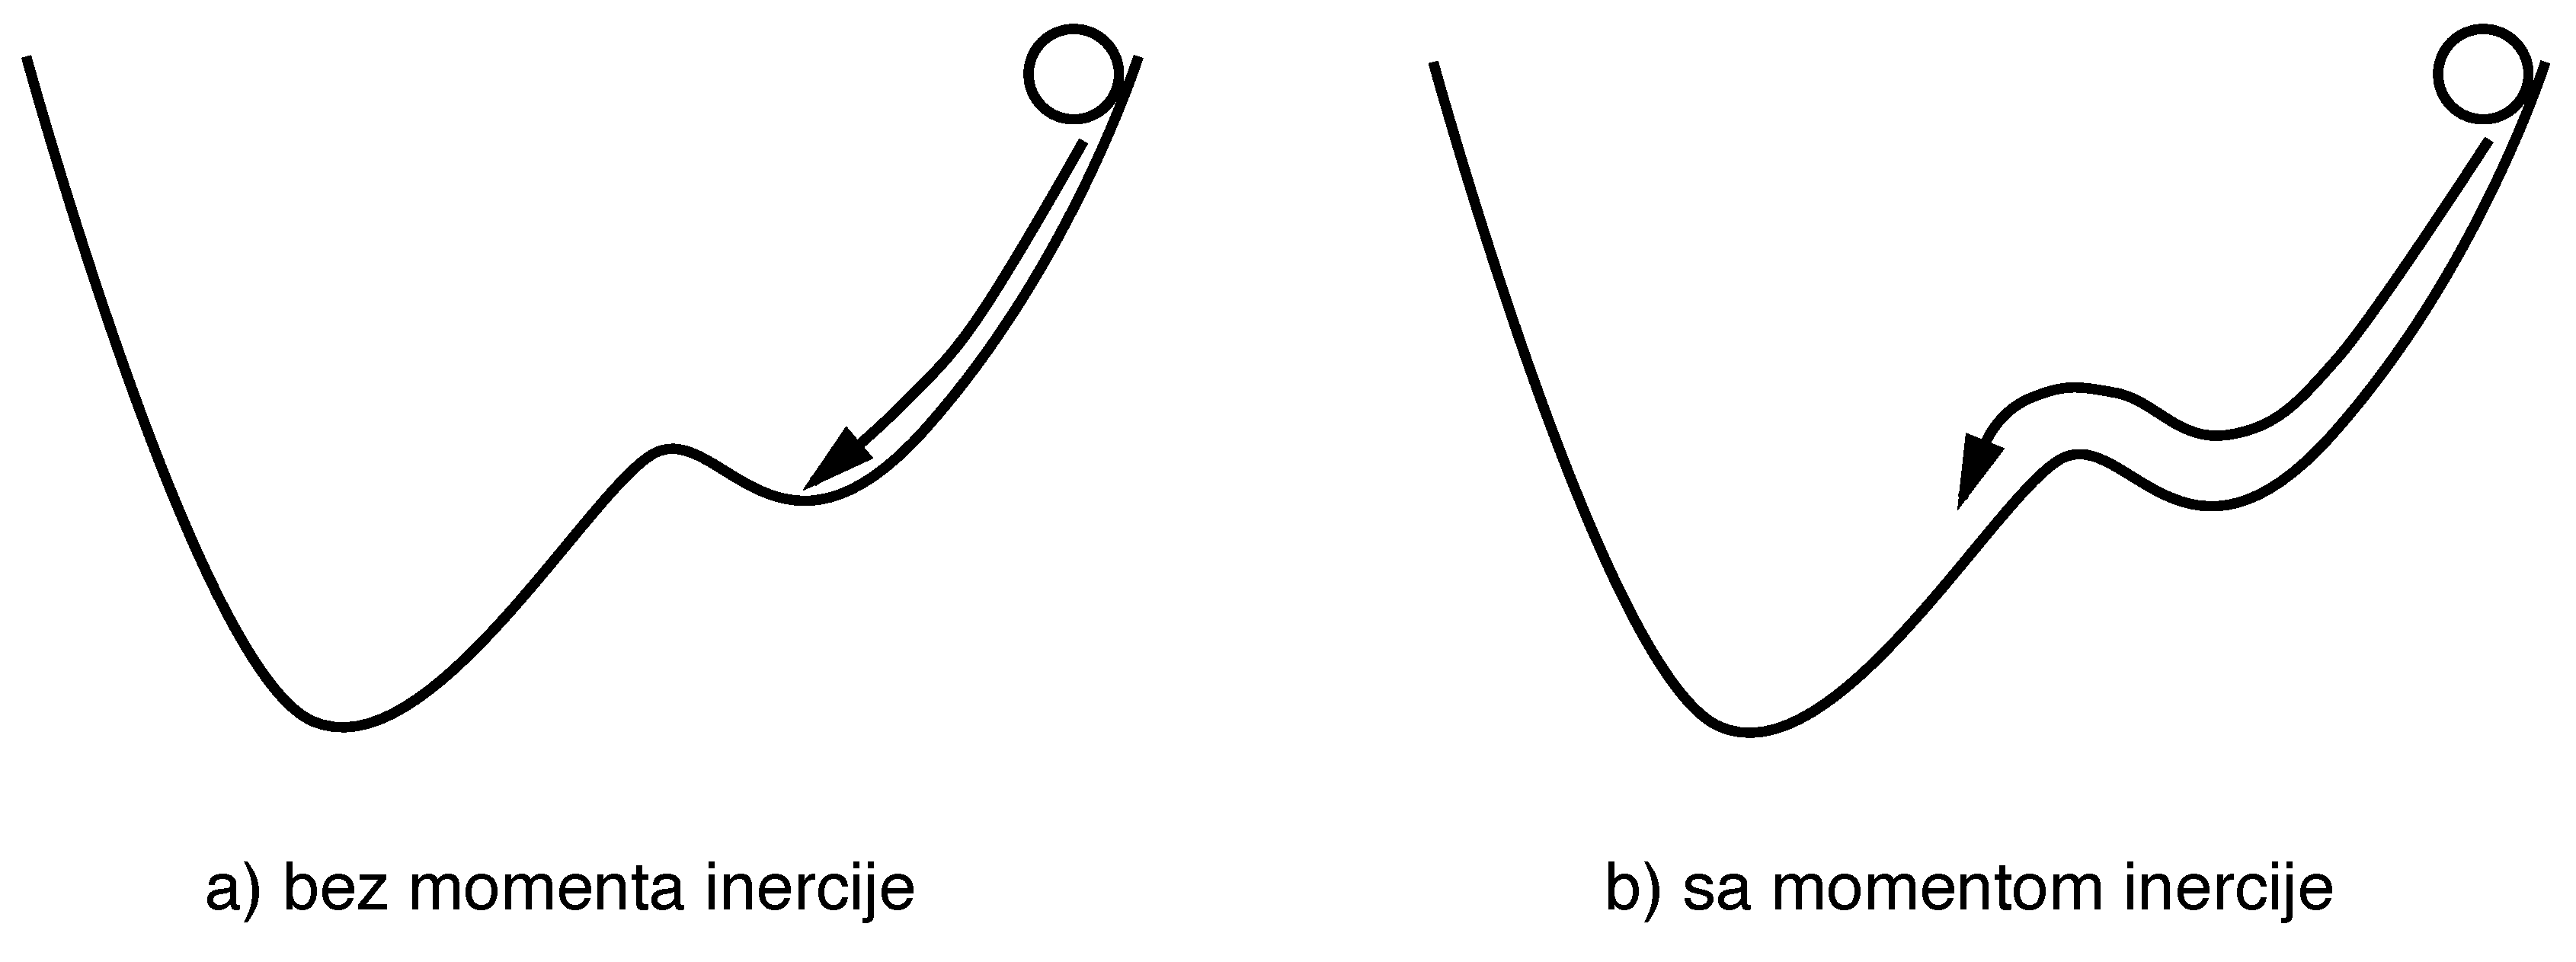
\includegraphics[width=14cm]{images/momentum.pdf}
    \caption{Učenje uz moment inercije}
    \label{fig:momentum}
\end{figure}

No ukoliko loptica ima moment inercije, ona će se nastaviti gibati te ako je lokalni minimum dovoljno malen, loptica će ga napustiti i nastaviti gibanje prema globalnom minimumu. Izraz za korekciju težina pri kojoj se koristi moment inercije je:$$w_{i,j}^{(k)} \leftarrow w_{i,j}^{(k)} + \eta\cdot y_i ^ {(k)}\cdot \delta_j^{(k+1)} + \alpha\cdot\Delta w_{i,j}^{(k)'},$$ gdje $\alpha$ predstavlja moment inercije, što je obično u intervalu od $0$ do $1$, te $\Delta w_{i,j}^{(k)'}$ predstavlja vrijednost korekcije iz prethodnog koraka.


\chapter{Izlučivanje značajki}
Nakon što su slike slova segmentirane i obrađene te je izabrana metoda klasifikacije višeslojnom potpuno povezanom unaprijednom neuronskom mrežom koja je učena s algoritmom propagacije pogreške unatrag s dodatkom momenta inercije, sljedeći korak je izlučivanje značajki iz pojedinog slova, to jest slike.

\section{Uvod}

Izlučivanje značajki iz skupa podataka, to jest iz slika slova, ključan je korak prilikom izgradnje sustava za automatsko prepoznavanje rukom pisanih slova. Sam uspjeh generalizacije pojedinog slova upravo ovisi o skupu značajki koje su izlučene iz slova. Ukoliko je vektor značajki pojedinog slova zadovoljavajući tada vektor značajki istog slova ne bi smio se previše razlikovati. No ukoliko je vektor značajki loš, to jest ne predstavlja ključne segmente nekog slova, tada će doći do rasipanja rezultata.

Kod značajki rukom pisanih slova, ali i kod računalno generiranih slova, postoje dvije vrste značajki: strukturalne i statističke značajke. Strukturne značajke predstavljaju strukturu samog slova i vrlo su otporne na stil pisanja i rukopis, to jest font u slučaju računalno generiranih slova. Strukturne značajke se obično temelje na geometrijskim i topološkim svojstvima slova kao što je omjer dužine i širine slova, broj presjecišta, petlji, grananja, krajnjih točaka i drugih.

Statističke značajke uzimaju u obzir statističku raspodjelu slikovnih elemenata i njihovu vrijednost. Često korištene statističke značajke su: podjela na zone, projekcijski histogrami, vertikalne i horizontalne projekcije te dijagonalne projekcije \citep{diagonal2011}.

Za potrebe ovog rada isprobane su vertikalne, horizontalne i dijagonalne projekcije iz skupa statističkih značajki te broj presjecišta i krajnjih točaka iz skupine strukturnih značajki i raznorazne hibridne kombinacije već navedenih značajki.

\section{Strukturne značajke}

Za izlučivanje strukturnih značajki korišten je strukturni element dimenzija \emph{3 x 3} prikazan na slici \ref{fig:points_kernel}. Element $P_1$ predstavlja središnji element kojim se vršila usporedba s originalnom slikom, to jest s pojedinim slikovnim elementom slova. Kako se navedeni strukturni element koristi nad binarnom slikom vrijednost elementa $P_i$ poprima vrijednost 0 ili 1, ovisno o tome je li slikovni element bijele ili crne boje. Bitno je napomenuti da se usporedbe i izračuni vrše samo u onom slučaju ukoliko je središnji element $P_1$ iznad crne točke. 

\begin{figure}[htb]
    \centering
    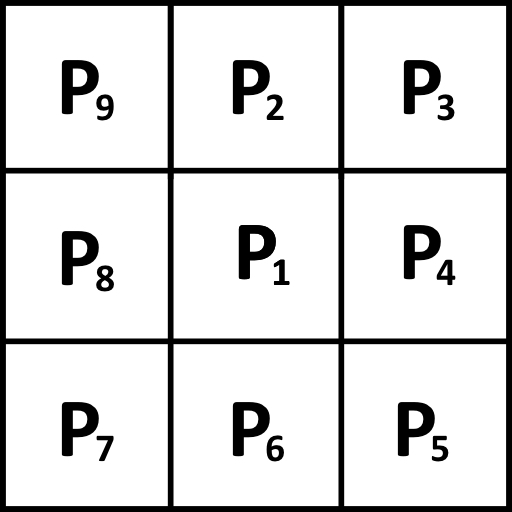
\includegraphics[width=4cm]{images/kernel.jpg}
    \caption{Strukturni element}
    \label{fig:points_kernel}
\end{figure}

Kako bi se trenutna crna točka nad kojom se nalazi strukturni element klasificirala kao krajnja točka nužno je zadovoljiti sljedeći uvjet:$$\sum_{i=2}^{9} P_i = 1.$$
Za klasifikaciju točke kao točke presjecišta nužno je zadovoljiti sljedeći jedan od sljedeća dva uvjeta:$$P_2 + P_4 + P_6 + P_8 \geq 2$$ ili $$P_3 + P_5 + P_7 + P_9 \geq 2.$$

Kako broj krajnjih točaka i točaka presjecišta može biti više, a neuronska mreža na svoje ulaze prima vrijednosti iz intervala od nula do jedan, u vektoru značajki se koristi njihova recipročna vrijednost, ili nula ukoliko navedenih točaka nema.

\section{Statističke značajke}

Od statističkih značajki korištene su horizontalna, vertikalna i dijagonala projekcija. Kao početna pozicija slike se gleda gornji lijevi ugao i ima koordinate $(1, 1)$.

\subsection{Horizontalna i vertikalna projekcije}

Za sliku, horizontalna projekcija je definirana nad svakim retkom kao skup od tri elementa:
\begin{enumerate}
    \item broj crnih slikovnih elemenata u pojedinom retku,
    \item pozicija prvog crnog slikovnog elementa s lijeva i
    \item pozicija prvog crnog slikovnog elementa s desna.
\end{enumerate}
Kako bi navedeni elementi bili neovisni o dimenziji slike, pojedini element se dijeli sa širinom slike, što uostalom postavlja dobivene brojeve u interval od nula do jedan, što zapravo savršeno odgovara kao ulaz neuronskoj mreži.

Što se tiče vertikalne projekcije, ona je definirana nad svakim stupcem slike kao skup od tri elementa:
\begin{enumerate}
    \item broj crnih slikovnih elemenata u pojedinom retku,
    \item pozicija prvog crnog slikovnog elementa od vrha i
    \item pozicija prvog crnog slikovnog elementa od dna.
\end{enumerate}
Iz istih razloga kao i kod horizontalne projekcije, pojedini element se dijeli sa visinom slike.

Na primjeru slike \ref{fig:hv_projection} za treći redak horizontalna projekcija bi bila $(0.5, 0.5, 0.83)$. Vertikalna projekcija za treći stupac bi bila $(0.16, 0.5, 0.5).$

\begin{figure}[htb]
    \centering
    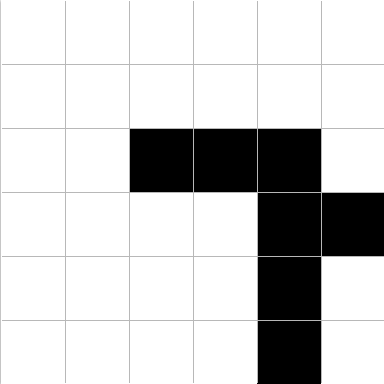
\includegraphics[width=5cm]{images/hvProj.png}
    \caption{Primjer za horizontalnu i vertikalnu projekciju}
    \label{fig:hv_projection}
\end{figure}

\subsection{Dijagonalna projekcija}

Dijagonalna projekcija je relativno nova tehnika izlučivanja značajki, koju su predstavili Pradeep, Srinivasan i Himavathi u svom radu 2011. godine  \citep{diagonal2011}.

Ulazna slika je dimenzija $30 \times 30$ točaka. Slika se zatim podjeli na 36 jednakih zona dimenzija $5 \times 5$. Svaka zona ima devet dijagonala i kretanjem po svakoj od dijagonala računa se koeficijent dijagonale tako da se broj točaka objekta, odnosno crnih točaka, dijeli s ukupnim brojem elemenata u toj dijagonali. Nakon što se prođu sve dijagonale u zoni, koeficijenti dijagonala se zbroje i podjele s ukupnim brojem dijagonala u zoni i na taj način se dobiva koeficijent pojedine zone. Primjer obilaska dijagonala dan je na slici \ref{fig:diagonals}.
\begin{figure}[htb]
    \centering
    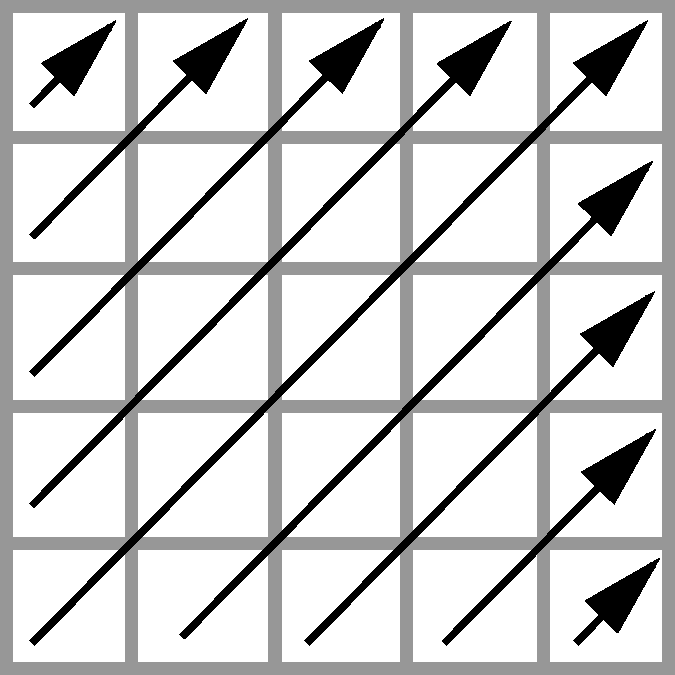
\includegraphics[width=5cm]{images/diagonal_arrows.pdf}
    \caption{Smjer obilaska dijagonala u zoni}
    \label{fig:diagonals}
\end{figure}

Uz navedenih 36 značajki, još se pridodaje 12 značajki koje računaju prosječni koeficijent zona za pojedini redak i pojedini stupac što ukupno daje 48 značajki za sliku dimenzija $30 \times 30$. Implementacija algoritma za izračunavanje koeficijenta pojedine zone u programskom jeziku \emph{Java} dana je sljedećim izvornim kodom.
\lstset{language=Java, tabsize=2}
\begin{lstlisting}
private double calculateZone(int[][] zone) {
    int count = 2 * ZONE_SIZE - 1;
    double sum = 0;
    for (int i = 0; i < count; i++) {
        int z = i < ZONE_SIZE ? 0 : i - ZONE_SIZE + 1;
        int sliceSize = i - z + 1;
        int sliceSum = 0;
        for (int j = z; j < sliceSize; j++)
            if (zone[j][i - j] == 1) sliceSum++;
        sum += sliceSum / (double) sliceSize;
    }
    return sum / count;
}
\end{lstlisting}


\chapter{Učenje i rezultati}
Kako je već navedeno, kao klasifikator korištena je višeslojna unaprijedna potpuno povezana neuronska mreža učena s algoritmom propagacije pogreške unatrag uz dodatak momenta inercije. Korištena je implementacija neuronske mreže iz biblioteke otvorenog koda \emph{Neuroph}\footnote{link: http://neuroph.sourceforge.net}. Prilikom učenja isprobano je više raznih parametara, od stope učenja, momenta inercije preko raznoraznih kombinacija broja neurona unutar skrivenih slojeva, pa i sam broj skrivenih slojeva. Najbolji rezultati su dobiveni za dva skrivena sloja po $86$ neurona u svakome od slojeva. Stopa učenja je bila $\eta = 0.01$, a moment inercije $\alpha = 0.025$.

Kao vektor značajki isprobano je niz kombinacija poput pojedinačne vertikalne, horizontalne i dijagonalne projekcije, pa hibridne kombinacije već navedenih. No na kraju je najbolje rezultate dala hibridna kombinacija dijagonalne i horizontalne projekcije te broja točaka presjecišta i krajnjih točaka. Točnije, slike su bile dimenzija $30 \times 30$ točaka pa je vektor značajki pojedine slike imao ukupno 65 elemenata. Od toga, dijagonalnoj projekciji je pripalo 48 elemenata, horizontalnoj projekciji 15 jer se u obzir uzimao svaki šesti redak slike te još po broj točaka presjecišta i broj krajnjih točaka na način kako je objašnjeno u prijašnjem poglavlju.

Kako se sustav koji se gradi kroz ovaj rad treba koristiti pri ispravljanju obrazaca s odgovorima za abc-pitalice krajnjem korisniku nije važna informacija je li ispitanik unio veliko ili malo slovo stoga je izlazni sloj neuronske mreže sadržavao 27 ili 32 izlaza, za pojedini razred slova, ovisno o tome je li se mreža učila na engleskoj ili hrvatskoj abecedi znakova. Abecedi znakova dodan je znak crtice '-' kao znak za poništavanje danog odgovora. Gledanje velikog i malog slova kao jedan razred ujedno je i olakšalo klasifikaciju neuronskoj mreži jer bez poznavanja konteksta mreža teško može razlikovati veliko i malo slovo o jer kad se skaliraju na istu dimenziju dobiju se dva ista slova.

Mreža je učena na hrvatskoj i engleskoj abecedi te na velikim i malim slovima. Najbolji rezultati su dobiveni za velika slova engleske abecede, dok su najlošiji dobiveni za velika i mala slova hrvatske abecede. U sljedećim tablicama prikazani su rezultati učenja za velika slova engleske abecede, te sva slova hrvatske abecede. Također radi usporedbe je prikazan i rezultat učenja vektorom horizontalne projekcije koji ima 90 elemenata te je učenje njime bilo dosta duže nego hibridnim vektorom. Stupac \emph{Metoda 1} predstavlja uspješnost prepoznavanja slova korištenjem vektora horizontalne projekcije, a stupac \emph{Metoda 2} predstavlja uspješnost prepoznavanja slova korištenjem hibridnog vektora dijagonalne i horizontalne projekcije i strukturnih točaka kako je već navedeno.  Pri testiranju mreže korišteno je po pet malih i pet velikih slova.

Što se tiče prikazanih rezultata za velika slova engleske abecede (tablica \ref{eng_abc}) i hibridnog vektora najviše je rasipanja rezultata na slovima Q, koje je mreža prepoznala kao O, no tu se nije moglo nešto previše napraviti jer u samom skupu podataka to slovo je ispisano s jako malom kvačicom na dnu, te na slovu N, koje je mreža prepoznala kao M, no to je također problem u samom skupu podataka. No u prikazanim podacima najviše odskače slovo H, kojeg mreža uz vektor horizontalne projekcije nije uspjela prepoznati niti jednom.

Kod rezultata hrvatske abecede (tablica \ref{cro_abc}) za velika i mala slova najviše problema stvaraju mala slova. Na primjer, malo slovo l je u potpunosti krivo klasificirano kao veliko slovo I.
Također, većina slova Č je klasificirana kao slovo Ć (slika \ref{fig:letter_ch}).
 \begin{figure}[htb]
    \centering
    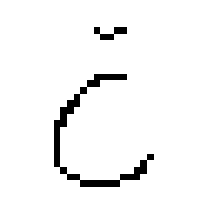
\includegraphics[width=4cm]{images/ch.png}
    \caption{Slovo č prepoznato kao slovo ć}
    \label{fig:letter_ch}
\end{figure}
Također su sva mala slova g prepoznata kao malo slovo q jer ih ljudi dosta slično pišu, što je i prikazano na slici \ref{fig:letter_g}.
 \begin{figure}[htb]
    \centering
    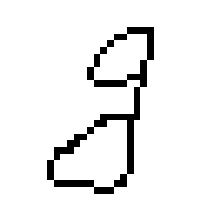
\includegraphics[width=4cm]{images/g.png}
    \caption{Malo slovo g prepoznato kao malo slovo q}
    \label{fig:letter_g}
\end{figure}
Navedeni problemi su vidljivi i kod vektora horizontalne projekcije i hibridnog vektora. No i tu problem leži u samom skupu podataka jer većina ljudi malo slovo l piše kao veliko slovo I, i to bez ikakve razlike, što je i prikazano na slici \ref{fig:letter_l}.
 \begin{figure}[htb]
    \centering
    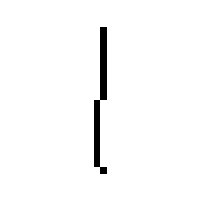
\includegraphics[width=4cm]{images/letter_l.png}
    \caption{Malo slovo l prepoznato kao veliko slovo I}
    \label{fig:letter_l}
\end{figure}
Zanimljivo je primijetiti kako je većina slova č krivo klasificirana, dok su sva slova ć uredno prepoznata. I tu je problem kod skupa podataka jer većina ljudi slovo č piše s jednom polegnutom kvačicom, što bez konteksta teško da se može znati o kom je slovu riječ pa to mreža klasificira kao ć. Bitno je napomenuti da je u tablici \ref{cro_abc} izostavljen rezultat prepoznavanja znaka poništavanja odgovora, to jest crtice, zbog ljepšeg formatiranja tablice, no njegovo prepoznavanje je u potpunosti točno. Matrica zabune za pojedino slovo hrvatske abecede prikazana je tablicom \ref{confusion_matrix_cro}, dok za velika slova engleske abecede je prikazana tablicom \ref{confusion_matrix_eng}.

\begin{table}[]
\centering
\caption{Broj prepoznatih velikih slova engleske abecede. Svako slovo je testirano s pet primjeraka.}
\label{eng_abc}
\begin{tabular}{c|c|c}
Slovo & Metoda 1 & Metoda 2 \\ \hline
A & 4/5 & 4/5 \\ \hline
B & 5/5 & 5/5 \\ \hline
C & 5/5 & 5/5 \\ \hline
D & 5/5 & 4/5 \\ \hline
E & 5/5 & 5/5 \\ \hline
F & 5/5 & 5/5 \\ \hline
G & 5/5 & 3/5 \\ \hline
H & 0/5 & 4/5 \\ \hline
I & 5/5 & 5/5 \\ \hline
J & 5/5 & 5/5 \\ \hline
K & 3/5 & 4/5 \\ \hline
L & 5/5 & 5/5 \\ \hline
M & 3/5 & 5/5 \\ \hline
N & 4/5 & 3/5 \\ \hline
O & 5/5 & 5/5 \\ \hline
P & 5/5 & 5/5 \\ \hline
R & 3/5 & 4/5 \\ \hline
S & 5/5 & 5/5 \\ \hline
T & 5/5 & 5/5 \\ \hline
U & 2/5 & 4/5 \\ \hline
V & 4/5 & 5/5 \\ \hline
Z & 5/5 & 4/5 \\ \hline
X & 4/5 & 4/5 \\ \hline
Y & 5/5 & 5/5 \\ \hline
W & 5/5 & 4/5 \\ \hline
Q & 3/5 & 2/5 \\ \hline
- & 5/5 & 5/5 \\ \hline
Uku. & 85.71\% & 88.57\%
\end{tabular}
\end{table}

\begin{table}[]
\centering
\caption{Broj prepoznatih velikih i malih slova hrvatske abecede. Svako slovo je testirano s deset primjeraka, to jest pet velikih i pet malih slova.}
\label{cro_abc}
\scalebox{0.95} {
\begin{tabular}{c|c|c}
\hline
Slovo & Metoda 1 & Metoda 2 \\ \hline
A & 6/10 & 7/10 \\ \hline
B & 9/10 & 10/10 \\ \hline
C & 10/10 & 9/10 \\ \hline
D & 7/10 & 6/10 \\ \hline
E & 9/10 & 9/10 \\ \hline
F & 5/10 & 6/10 \\ \hline
G & 7/10 & 4/10 \\ \hline
H & 3/10 & 8/10 \\ \hline
I & 8/10 & 9/10 \\ \hline
J & 10/10 & 10/10 \\ \hline
K & 6/10 & 8/10 \\ \hline
L & 5/10 & 5/10 \\ \hline
M & 8/10 & 9/10 \\ \hline
N & 5/10 & 6/10 \\ \hline
O & 10/10 & 9/10 \\ \hline
P & 10/10 & 10/10 \\ \hline
R & 9/10 & 8/10 \\ \hline
S & 10/10 & 9/10 \\ \hline
T & 10/10 & 10/10 \\ \hline
U & 7/10 & 8/10 \\ \hline
V & 9/10 & 10/10 \\ \hline
Z & 9/10 & 8/10 \\ \hline
X & 6/10 & 9/10 \\ \hline
Y & 10/10 & 10/10 \\ \hline
W & 9/10 & 9/10 \\ \hline
Q & 3/10 & 3/10 \\ \hline
Č & 2/10 & 2/10 \\ \hline
Ć & 10/10 & 10/10 \\ \hline
Đ & 9/10 & 10/10 \\ \hline
Š & 8/10 & 5/10 \\ \hline
Ž & 7/10 & 6/10 \\ \hline
Uku. & 76.88\% & 78.44\% \\ \hline
\end{tabular}
}
\end{table}


\begin{table}[]
\setlength{\tabcolsep}{2pt}
\centering
\caption{Matrica zabune za hrvatsku abecedu. Element tablice predstavlja broj koliko je puta slovo iz retka prepoznato kao slovo iz stupca. Svako slovo je testirano s deset primjeraka.}
\label{confusion_matrix_cro}
\scalebox{0.9} {
\begin{tabular}{c|c|c|c|c|c|c|c|c|c|c|c|c|c|c|c|c|c|c|c|c|c|c|c|c|c|c|c|c|c|c|c|c}
\cline{2-33}
  & A & B  & C & D & E & F & G & H & I & J  & K & L & M & N & O & P  & R & S & T  & U & V  & Z & X & Y  & W & Q & Č & Ć  & Đ  & Š & Ž & -  \\ \hline
A & 7 & 0  & 0 & 0 & 0 & 0 & 1 & 0 & 0 & 0  & 0 & 0 & 0 & 0 & 0 & 0  & 0 & 0 & 0  & 0 & 0  & 0 & 0 & 1  & 0 & 0 & 0 & 0  & 1  & 0 & 0 & 0  \\ \hline
B & 0 & 10 & 0 & 0 & 0 & 0 & 0 & 0 & 0 & 0  & 0 & 0 & 0 & 0 & 0 & 0  & 0 & 0 & 0  & 0 & 0  & 0 & 0 & 0  & 0 & 0 & 0 & 0  & 0  & 0 & 0 & 0  \\ \hline
C & 0 & 0  & 9 & 0 & 0 & 0 & 0 & 0 & 0 & 0  & 0 & 0 & 0 & 1 & 0 & 0  & 0 & 0 & 0  & 0 & 0  & 0 & 0 & 0  & 0 & 0 & 0 & 0  & 0  & 0 & 0 & 0  \\ \hline
D & 0 & 1  & 0 & 6 & 0 & 0 & 0 & 0 & 0 & 0  & 1 & 0 & 0 & 0 & 0 & 0  & 0 & 0 & 0  & 1 & 0  & 0 & 1 & 0  & 0 & 0 & 0 & 0  & 0  & 0 & 0 & 0  \\ \hline
E & 0 & 0  & 0 & 0 & 9 & 0 & 0 & 0 & 0 & 0  & 0 & 1 & 0 & 0 & 0 & 0  & 0 & 0 & 0  & 0 & 0  & 0 & 0 & 0  & 0 & 0 & 0 & 0  & 0  & 0 & 0 & 0  \\ \hline
F & 0 & 0  & 0 & 0 & 0 & 6 & 0 & 0 & 0 & 0  & 0 & 0 & 0 & 0 & 0 & 2  & 0 & 0 & 0  & 0 & 0  & 0 & 0 & 2  & 0 & 0 & 0 & 0  & 0  & 0 & 0 & 0  \\ \hline
G & 1 & 0  & 0 & 0 & 0 & 0 & 4 & 0 & 0 & 0  & 0 & 0 & 0 & 0 & 0 & 1  & 0 & 0 & 0  & 0 & 0  & 0 & 0 & 0  & 0 & 4 & 0 & 0  & 0  & 0 & 0 & 0  \\ \hline
H & 0 & 0  & 0 & 0 & 0 & 0 & 0 & 8 & 0 & 0  & 0 & 0 & 0 & 2 & 0 & 0  & 0 & 0 & 0  & 0 & 0  & 0 & 0 & 0  & 0 & 0 & 0 & 0  & 0  & 0 & 0 & 0  \\ \hline
I & 0 & 0  & 0 & 0 & 0 & 0 & 0 & 0 & 9 & 0  & 0 & 1 & 0 & 0 & 0 & 0  & 0 & 0 & 0  & 0 & 0  & 0 & 0 & 0  & 0 & 0 & 0 & 0  & 0  & 0 & 0 & 0  \\ \hline
J & 0 & 0  & 0 & 0 & 0 & 0 & 0 & 0 & 0 & 10 & 0 & 0 & 0 & 0 & 0 & 0  & 0 & 0 & 0  & 0 & 0  & 0 & 0 & 0  & 0 & 0 & 0 & 0  & 0  & 0 & 0 & 0  \\ \hline
K & 0 & 0  & 0 & 0 & 0 & 0 & 0 & 0 & 1 & 0  & 8 & 0 & 0 & 0 & 0 & 0  & 0 & 0 & 0  & 0 & 0  & 0 & 0 & 0  & 0 & 0 & 0 & 0  & 0  & 1 & 0 & 0  \\ \hline
L & 0 & 0  & 0 & 0 & 0 & 0 & 0 & 0 & 5 & 0  & 0 & 5 & 0 & 0 & 0 & 0  & 0 & 0 & 0  & 0 & 0  & 0 & 0 & 0  & 0 & 0 & 0 & 0  & 0  & 0 & 0 & 0  \\ \hline
M & 0 & 0  & 0 & 0 & 0 & 0 & 0 & 1 & 0 & 0  & 0 & 0 & 9 & 0 & 0 & 0  & 0 & 0 & 0  & 0 & 0  & 0 & 0 & 0  & 0 & 0 & 0 & 0  & 0  & 0 & 0 & 0  \\ \hline
N & 0 & 0  & 0 & 0 & 0 & 0 & 0 & 0 & 0 & 0  & 0 & 0 & 1 & 6 & 0 & 0  & 1 & 0 & 0  & 1 & 0  & 0 & 1 & 0  & 0 & 0 & 0 & 0  & 0  & 0 & 0 & 0  \\ \hline
O & 0 & 0  & 0 & 0 & 0 & 0 & 0 & 0 & 0 & 0  & 0 & 0 & 0 & 0 & 9 & 0  & 0 & 0 & 0  & 0 & 0  & 0 & 0 & 0  & 1 & 0 & 0 & 0  & 0  & 0 & 0 & 0  \\ \hline
P & 0 & 0  & 0 & 0 & 0 & 0 & 0 & 0 & 0 & 0  & 0 & 0 & 0 & 0 & 0 & 10 & 0 & 0 & 0  & 0 & 0  & 0 & 0 & 0  & 0 & 0 & 0 & 0  & 0  & 0 & 0 & 0  \\ \hline
R & 0 & 0  & 0 & 0 & 0 & 0 & 0 & 0 & 0 & 0  & 0 & 2 & 0 & 0 & 0 & 0  & 8 & 0 & 0  & 0 & 0  & 0 & 0 & 0  & 0 & 0 & 0 & 0  & 0  & 0 & 0 & 0  \\ \hline
S & 0 & 0  & 0 & 0 & 1 & 0 & 0 & 0 & 0 & 0  & 0 & 0 & 0 & 0 & 0 & 0  & 0 & 9 & 0  & 0 & 0  & 0 & 0 & 0  & 0 & 0 & 0 & 0  & 0  & 0 & 0 & 0  \\ \hline
T & 0 & 0  & 0 & 0 & 0 & 0 & 0 & 0 & 0 & 0  & 0 & 0 & 0 & 0 & 0 & 0  & 0 & 0 & 10 & 0 & 0  & 0 & 0 & 0  & 0 & 0 & 0 & 0  & 0  & 0 & 0 & 0  \\ \hline
U & 0 & 0  & 0 & 0 & 0 & 0 & 0 & 0 & 0 & 0  & 0 & 0 & 0 & 0 & 0 & 0  & 0 & 0 & 0  & 8 & 2  & 0 & 0 & 0  & 0 & 0 & 0 & 0  & 0  & 0 & 0 & 0  \\ \hline
V & 0 & 0  & 0 & 0 & 0 & 0 & 0 & 0 & 0 & 0  & 0 & 0 & 0 & 0 & 0 & 0  & 0 & 0 & 0  & 0 & 10 & 0 & 0 & 0  & 0 & 0 & 0 & 0  & 0  & 0 & 0 & 0  \\ \hline
Z & 0 & 0  & 0 & 0 & 0 & 0 & 0 & 0 & 0 & 0  & 0 & 0 & 0 & 0 & 0 & 0  & 1 & 0 & 0  & 0 & 0  & 8 & 0 & 0  & 0 & 0 & 0 & 0  & 0  & 0 & 1 & 0  \\ \hline
X & 0 & 0  & 0 & 0 & 0 & 0 & 0 & 0 & 0 & 0  & 1 & 0 & 0 & 0 & 0 & 0  & 0 & 0 & 0  & 0 & 0  & 0 & 9 & 0  & 0 & 0 & 0 & 0  & 0  & 0 & 0 & 0  \\ \hline
Y & 0 & 0  & 0 & 0 & 0 & 0 & 0 & 0 & 0 & 0  & 0 & 0 & 0 & 0 & 0 & 0  & 0 & 0 & 0  & 0 & 0  & 0 & 0 & 10 & 0 & 0 & 0 & 0  & 0  & 0 & 0 & 0  \\ \hline
W & 0 & 0  & 0 & 0 & 0 & 0 & 0 & 0 & 0 & 1  & 0 & 0 & 0 & 0 & 0 & 0  & 0 & 0 & 0  & 0 & 0  & 0 & 0 & 0  & 9 & 0 & 0 & 0  & 0  & 0 & 0 & 0  \\ \hline
Q & 0 & 0  & 0 & 0 & 0 & 0 & 4 & 0 & 0 & 0  & 0 & 0 & 0 & 0 & 3 & 0  & 0 & 0 & 0  & 0 & 0  & 0 & 0 & 0  & 0 & 3 & 0 & 0  & 0  & 0 & 0 & 0  \\ \hline
Č & 0 & 0  & 0 & 0 & 0 & 0 & 0 & 0 & 0 & 0  & 0 & 0 & 0 & 0 & 0 & 0  & 0 & 0 & 0  & 0 & 0  & 0 & 0 & 0  & 0 & 0 & 2 & 8  & 0  & 0 & 0 & 0  \\ \hline
Ć & 0 & 0  & 0 & 0 & 0 & 0 & 0 & 0 & 0 & 0  & 0 & 0 & 0 & 0 & 0 & 0  & 0 & 0 & 0  & 0 & 0  & 0 & 0 & 0  & 0 & 0 & 0 & 10 & 0  & 0 & 0 & 0  \\ \hline
Đ & 0 & 0  & 0 & 0 & 0 & 0 & 0 & 0 & 0 & 0  & 0 & 0 & 0 & 0 & 0 & 0  & 0 & 0 & 0  & 0 & 0  & 0 & 0 & 0  & 0 & 0 & 0 & 0  & 10 & 0 & 0 & 0  \\ \hline
Š & 0 & 0  & 0 & 0 & 0 & 1 & 0 & 0 & 0 & 1  & 0 & 0 & 0 & 0 & 0 & 0  & 0 & 0 & 0  & 0 & 0  & 0 & 0 & 1  & 0 & 0 & 0 & 2  & 0  & 5 & 0 & 0  \\ \hline
Ž & 0 & 0  & 0 & 0 & 0 & 1 & 0 & 0 & 0 & 0  & 0 & 0 & 0 & 0 & 0 & 0  & 0 & 0 & 0  & 0 & 0  & 0 & 0 & 0  & 1 & 0 & 1 & 0  & 0  & 1 & 6 & 0  \\ \hline
- & 0 & 0  & 0 & 0 & 0 & 0 & 0 & 0 & 0 & 0  & 0 & 0 & 0 & 0 & 0 & 0  & 0 & 0 & 0  & 0 & 0  & 0 & 0 & 0  & 0 & 0 & 0 & 0  & 0  & 0 & 0 & 10 \\ \hline
\end{tabular}
}
\end{table}


\begin{table}[]
\setlength{\tabcolsep}{2pt}
\centering
\caption{Matrica zabune za velika slova engleske abecede. Element tablice predstavlja broj koliko je puta slovo iz retka prepoznato kao slovo iz stupca. Svako slovo je testirano s pet primjeraka.}
\label{confusion_matrix_eng}
\begin{tabular}{c|c|c|c|c|c|c|c|c|c|c|c|c|c|c|c|c|c|c|c|c|c|c|c|c|c|c|c}
\cline{2-28}
  & A & B & C & D & E & F & G & H & I & J & K & L & M & N & O & P & R & S & T & U & V & Z & X & Y & W & Q & - \\ \hline
A & 4 & 0 & 0 & 0 & 0 & 0 & 0 & 0 & 0 & 0 & 0 & 0 & 0 & 0 & 0 & 0 & 0 & 0 & 0 & 0 & 0 & 0 & 0 & 1 & 0 & 0 & 0 \\ \hline
B & 0 & 5 & 0 & 0 & 0 & 0 & 0 & 0 & 0 & 0 & 0 & 0 & 0 & 0 & 0 & 0 & 0 & 0 & 0 & 0 & 0 & 0 & 0 & 0 & 0 & 0 & 0 \\ \hline
C & 0 & 0 & 5 & 0 & 0 & 0 & 0 & 0 & 0 & 0 & 0 & 0 & 0 & 0 & 0 & 0 & 0 & 0 & 0 & 0 & 0 & 0 & 0 & 0 & 0 & 0 & 0 \\ \hline
D & 0 & 1 & 0 & 4 & 0 & 0 & 0 & 0 & 0 & 0 & 0 & 0 & 0 & 0 & 0 & 0 & 0 & 0 & 0 & 0 & 0 & 0 & 0 & 0 & 0 & 0 & 0 \\ \hline
E & 0 & 0 & 0 & 0 & 5 & 0 & 0 & 0 & 0 & 0 & 0 & 0 & 0 & 0 & 0 & 0 & 0 & 0 & 0 & 0 & 0 & 0 & 0 & 0 & 0 & 0 & 0 \\ \hline
F & 0 & 0 & 0 & 0 & 0 & 5 & 0 & 0 & 0 & 0 & 0 & 0 & 0 & 0 & 0 & 0 & 0 & 0 & 0 & 0 & 0 & 0 & 0 & 0 & 0 & 0 & 0 \\ \hline
G & 0 & 0 & 0 & 0 & 0 & 0 & 3 & 0 & 0 & 0 & 0 & 0 & 0 & 0 & 1 & 0 & 0 & 0 & 0 & 0 & 0 & 0 & 0 & 0 & 0 & 1 & 0 \\ \hline
H & 0 & 0 & 0 & 0 & 0 & 0 & 0 & 4 & 0 & 0 & 0 & 0 & 0 & 0 & 0 & 0 & 0 & 0 & 0 & 0 & 0 & 0 & 1 & 0 & 0 & 0 & 0 \\ \hline
I & 0 & 0 & 0 & 0 & 0 & 0 & 0 & 0 & 5 & 0 & 0 & 0 & 0 & 0 & 0 & 0 & 0 & 0 & 0 & 0 & 0 & 0 & 0 & 0 & 0 & 0 & 0 \\ \hline
J & 0 & 0 & 0 & 0 & 0 & 0 & 0 & 0 & 0 & 5 & 0 & 0 & 0 & 0 & 0 & 0 & 0 & 0 & 0 & 0 & 0 & 0 & 0 & 0 & 0 & 0 & 0 \\ \hline
K & 0 & 0 & 0 & 0 & 0 & 0 & 0 & 0 & 0 & 0 & 4 & 0 & 0 & 0 & 0 & 0 & 1 & 0 & 0 & 0 & 0 & 0 & 0 & 0 & 0 & 0 & 0 \\ \hline
L & 0 & 0 & 0 & 0 & 0 & 0 & 0 & 0 & 0 & 0 & 0 & 5 & 0 & 0 & 0 & 0 & 0 & 0 & 0 & 0 & 0 & 0 & 0 & 0 & 0 & 0 & 0 \\ \hline
M & 0 & 0 & 0 & 0 & 0 & 0 & 0 & 0 & 0 & 0 & 0 & 0 & 5 & 0 & 0 & 0 & 0 & 0 & 0 & 0 & 0 & 0 & 0 & 0 & 0 & 0 & 0 \\ \hline
N & 1 & 0 & 0 & 0 & 0 & 0 & 0 & 0 & 0 & 0 & 0 & 0 & 1 & 3 & 0 & 0 & 0 & 0 & 0 & 0 & 0 & 0 & 0 & 0 & 0 & 0 & 0 \\ \hline
O & 0 & 0 & 0 & 0 & 0 & 0 & 0 & 0 & 0 & 0 & 0 & 0 & 0 & 0 & 5 & 0 & 0 & 0 & 0 & 0 & 0 & 0 & 0 & 0 & 0 & 0 & 0 \\ \hline
P & 0 & 0 & 0 & 0 & 0 & 0 & 0 & 0 & 0 & 0 & 0 & 0 & 0 & 0 & 0 & 5 & 0 & 0 & 0 & 0 & 0 & 0 & 0 & 0 & 0 & 0 & 0 \\ \hline
R & 1 & 0 & 0 & 0 & 0 & 0 & 0 & 0 & 0 & 0 & 0 & 0 & 0 & 0 & 0 & 0 & 4 & 0 & 0 & 0 & 0 & 0 & 0 & 0 & 0 & 0 & 0 \\ \hline
S & 0 & 0 & 0 & 0 & 0 & 0 & 0 & 0 & 0 & 0 & 0 & 0 & 0 & 0 & 0 & 0 & 0 & 5 & 0 & 0 & 0 & 0 & 0 & 0 & 0 & 0 & 0 \\ \hline
T & 0 & 0 & 0 & 0 & 0 & 0 & 0 & 0 & 0 & 0 & 0 & 0 & 0 & 0 & 0 & 0 & 0 & 0 & 5 & 0 & 0 & 0 & 0 & 0 & 0 & 0 & 0 \\ \hline
U & 0 & 0 & 0 & 0 & 0 & 0 & 0 & 0 & 0 & 0 & 0 & 0 & 0 & 1 & 0 & 0 & 0 & 0 & 0 & 4 & 0 & 0 & 0 & 0 & 0 & 0 & 0 \\ \hline
V & 0 & 0 & 0 & 0 & 0 & 0 & 0 & 0 & 0 & 0 & 0 & 0 & 0 & 0 & 0 & 0 & 0 & 0 & 0 & 0 & 5 & 0 & 0 & 0 & 0 & 0 & 0 \\ \hline
Z & 0 & 0 & 0 & 0 & 0 & 0 & 0 & 0 & 0 & 1 & 0 & 0 & 0 & 0 & 0 & 0 & 0 & 0 & 0 & 0 & 0 & 4 & 0 & 0 & 0 & 0 & 0 \\ \hline
X & 0 & 0 & 0 & 0 & 0 & 0 & 0 & 0 & 0 & 0 & 1 & 0 & 0 & 0 & 0 & 0 & 0 & 0 & 0 & 0 & 0 & 0 & 4 & 0 & 0 & 0 & 0 \\ \hline
Y & 0 & 0 & 0 & 0 & 0 & 0 & 0 & 0 & 0 & 0 & 0 & 0 & 0 & 0 & 0 & 0 & 0 & 0 & 0 & 0 & 0 & 0 & 0 & 5 & 0 & 0 & 0 \\ \hline
W & 0 & 0 & 0 & 0 & 0 & 0 & 0 & 0 & 0 & 0 & 0 & 1 & 0 & 0 & 0 & 0 & 0 & 0 & 0 & 0 & 0 & 0 & 0 & 0 & 4 & 0 & 0 \\ \hline
Q & 0 & 0 & 0 & 0 & 0 & 0 & 0 & 0 & 0 & 0 & 0 & 0 & 0 & 0 & 3 & 0 & 0 & 0 & 0 & 0 & 0 & 0 & 0 & 0 & 0 & 2 & 0 \\ \hline
- & 0 & 0 & 0 & 0 & 0 & 0 & 0 & 0 & 0 & 0 & 0 & 0 & 0 & 0 & 0 & 0 & 0 & 0 & 0 & 0 & 0 & 0 & 0 & 0 & 0 & 0 & 5 \\ \hline
\end{tabular}
\end{table}

\chapter{Zaključak}
Tehnika prepoznavanja tiskanih i rukom pisanih slova se razvija još od polovice prošlog stoljeća i od tada je u mnogočemu evoluirala. U ovom radu, kao klasifikator pojedinog slova, korištena je višeslojna unaprijedna potpuno povezana neuronska mreža učena s algoritmom propagacije pogreške unatrag uz dodatak momenta inercije.

U radu je predstavljen cjeloviti postupak obrade slike kako bi se ulazna slika pripremila za izlučivanje značajki i učenje mreže. Kao vektor značajki korišten je hibridni vektor sastavljen od dijagonalne i horizontalne projekcije te broja presjecišta i broja krajnjih točaka.

Dobiveni rezultati su u granicama očekivanoga za dani skup podataka. U budućnosti bi se mogao proširiti skup podataka za zahtjevniju uporabu (trenutno se sastoji od 4480 slova). Također, kao klasifikator bi se mogla isprobati i duboka konvolucijska neuronska mreža koja problem prepoznavanja znamenaka rješava s točnošću od preko $99.7$\% \citep{umjint}.

\bibliography{literatura}
\bibliographystyle{fer}

\begin{sazetak}
U ovom radu prikazan je način rada i implementacija sustav za očitavanje rukom pisanih slova koji je projektiran tako da na svoj ulaz primi sliku slova, a na svom izlazu vrati prepoznato slovo. Primljena slika se obrađuje te se iz nje izdvaja kostur slova. Izvučeni kostur se zatim skalira na uniformne dimenzije i gradi se vektor značajki korištenjem dijagonalne i horizontalne projekcije te broja točaka presjecište i broja krajnjih točaka. Tako dobiveni vektor značajki se dovodi na ulaze neuronske mreže koja je učena algoritmom propagacije pogreške unatrag uz dodatak momenta inercije. Skup za učenje neuronske mreže se sastojao od 4480 velikih i malih tiskanih slova hrvatske i engleske abecede.

\kljucnerijeci{neuronske mreže, raspoznavanje rukom pisanih slova, obrada slike, binarizacija, dilatacija, stanjivanje, algoritam propagacije pogreške unatrag uz dodatak momenta inercije}
\end{sazetak}

% TODO: Navedite naslov na engleskom jeziku.
\engtitle{Handwritten Letters Recognition}
\begin{abstract}
This thesis describes the algorithm and implementation details of system for handwritten letter recognition. On its input, it receives letter image, and returns recognized letter as output. First, the input image is preprocessed and letter skeleton is extracted. After that, letter skeleton is scaled to uniform dimension and feature vector is extracted using diagonal and horizontal projection and number of cross-points and end-points. Extracted feature vector is input for neural network which is trained using backpropagation algorithm with momentum. Training set is consisted of 4480 large and small handwritten letters of Croatian and English alphabet.

\keywords{neural networks, handwritten letters recognition, image processing, binarization, dilation, thinning, backpropagation with momentum}
\end{abstract}

\end{document}